% DUNE experiment
% Target length: 25 pages

\graphicspath{{DUNE/Figs/}}

\chapter{The Deep Underground Neutrino Experiment}\label{chap:DUNE}

The Deep Underground Neutrino Experiment (DUNE) experiment \cite{DUNECDR1,DUNECDR2,DUNECDR3,DUNECDR4} is a future long-baseline neutrino experiment with a diverse physics program hosted by Fermilab, IL, U.S..  The far detector will be at the Sanford Underground Research Facility (SURF) near Lead, South Dakota, providing a baseline of 1300~km.  A cartoon of the experiment is shown in Figure~\ref{fig:DUNE}.

\begin{figure}
  \centering
  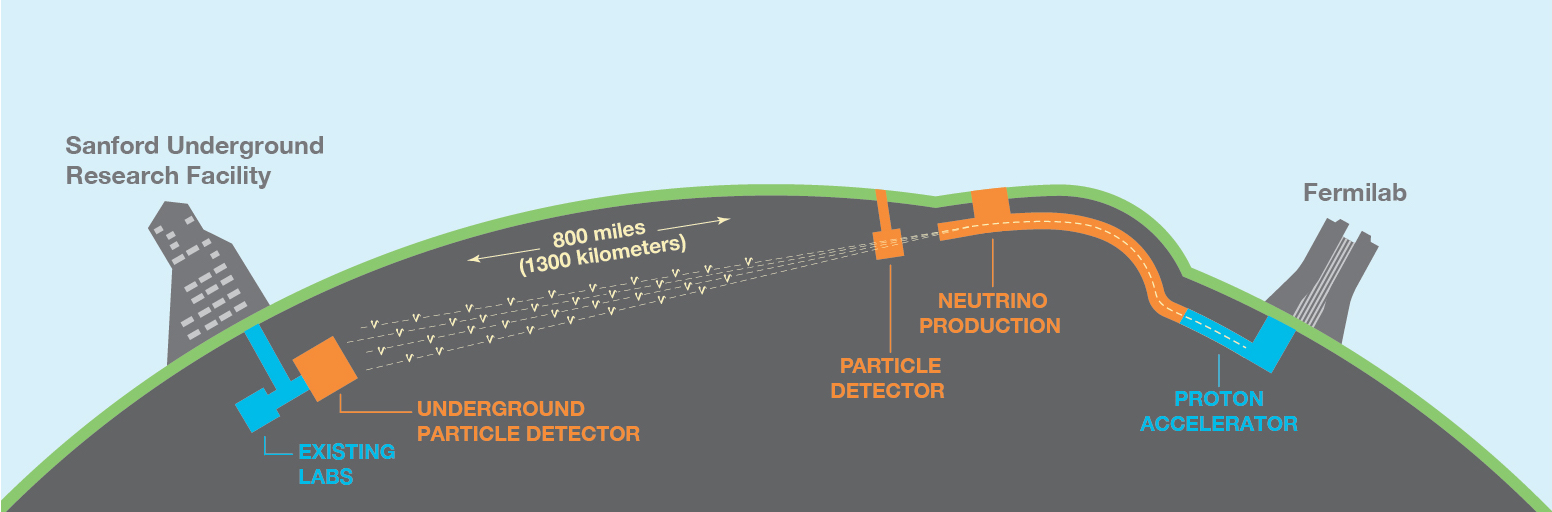
\includegraphics[width=14cm]{DUNE.jpg}
  \caption[Cartoon showing the configuration of the Deep Underground Neutrino Experiment.]{Cartoon showing the configuration of the Deep Underground Neutrino Experiment.  The experiment will be based at Fermilab, shown at the right of the figure, and will send neutrinos towards SURF, at the left hand side.  The distance travelled, through the Earth's crust, will be 1300~km.}
  \label{fig:DUNE}
\end{figure}

The DUNE experiment will be discussed in this present chapter.  As the experiment utilises liquid argon TPCs, a brief history and description of this detector technology is provided as a basis in Section~\ref{sec:LArTPC}.  An overview of the experiment, including its motivation, will be presented in Section~\ref{sec:DUNEOverview} before the experimental details are discussed in Section~\ref{sec:DUNEExperiment}.  The sensitivities of the experiment and its potential discoveries are the subject of Section~\ref{sec:DUNEPhysics}.  Finally, the schedule and strategy implemented by the collaboration to ensure commencement of data taking in around ten years' time is outlined in Section~\ref{sec:RoadToDUNE}.

%----------------------------------------------------------------------------------------------------------------------------------------------------------------------------
\section{The LAr TPC Concept}\label{sec:LArTPC}

The use of a liquid argon (LAr) Time Projection Chamber (TPC), or LArTPC, as a high-precision fine-grained detector medium holds much promise for the successful resolution of the open questions in neutrino physics.  A great amount of R\&D work has taken place to advance the maturity of the technology and pioneering experiments, such as ICARUS \cite{ICARUS2004}, have further increased the understanding of the neutrino community of the detector techniques.  Past and currently running experiments at Fermilab, such as ArgoNeuT \cite{ArgoNeuT2012}, LArIAT \cite{LArIAT2014} and MicroBooNE \cite{MicroBooNE2017}, are successfully using LArTPCs to take and analyse data and it seems certain to be the future of neutrino physics in the U.S. \cite{Baller2014}.

This section will provide a brief history of LArTPC technology and motivate its potential when used in a large experiment such as DUNE.  The basic operation of such a detector will also be described to provide background for discussion of the DUNE and 35~ton experiments, and of reconstruction in LArTPCs, in future chapters.

%----------------------------------------------------------------------------------------------------------------------------------------------------------------------------
\subsection{A Brief History of Time (Projection Chambers)}\label{sec:LArTPCHistory}

The use of a time projection chamber as a potential particle detector was put forward by David Nygren in 1974 \cite{Nygren1974}.  He envisioned bubble-chamber quality data but with the possibility of digital readout of the data, facilitating extremely fine spatial resolution, good timing resolution and fast recovery after triggering.  The basic concept is a drift chamber containing a noble gas placed within a field to drift ionisation electrons created by a propagating particle towards a multielectron array.  This setup allows full three-dimensional reconstruction by combining information from the two-dimensional readout plane with the drift time.  Nygren also included a magnetic field to assist particle identification in his design, shown in Figure~\ref{fig:NygrenTPC}.

\begin{figure}
  \centering
  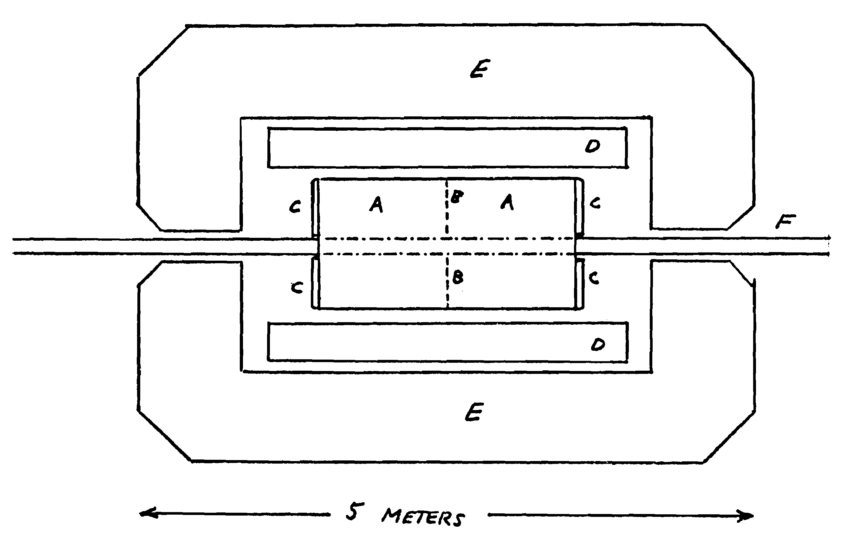
\includegraphics[width=10cm]{NygrenTPC.png}
  \caption[Original TPC design, Nygren (1974)]{The original concept of the time projection chamber particle detector, drawn by David Nygren in 1974 \cite{Nygren1974}.  The sections are labelled as followed: methane-filled region (A), screen to establish electron field (B), end-cap detectors (C), superconducting solenoid (3.33~T) (D), iron return yoke for magnetic field (E), beam vacuum pipe (F).}
  \label{fig:NygrenTPC}
\end{figure}

The extension of this concept to a liquid argon TPC and its potential as a high-precision fine-grained detector medium in neutrino physics was proposed by Carlo Rubbia in 1977 \cite{Rubbia1977}.  The use of a noble liquid rather than gas is necessary in neutrino experiments to provide a high enough target mass for increased probability of neutrino interactions.  Noble liquids have high electron mobility and low diffusion, favourable properties as the detection of particles is from the ionisation and scintillation light created by the particles.  Given the necessity of a high electric field in order to drift these electrons to the readout places, excellent dielectric properties are also required; noble liquids possess such qualities.  The properties of liquid argon which make it almost perfect for this use are demonstrated in Table~\ref{tab:NobleProperties}.

\begin{table}
  \caption{Properties of noble liquids relevant when considering a TPC medium for a neutrino experiment \cite{Soderberg2008}.}
  \label{tab:NobleProperties}
  \centering
  \begin{tabular}{ l c c c c c c }
    \toprule
     & Water & He & Ne & \color{red} Ar & Kr & Xe \\
    \midrule
    Boiling point [K] @ 1 atm & 373 & 4.2 & 27.1 & \color{red} 87.3 & 120.0 & 165.0 \\
    Density [g/cm$^3$] & 1 & 0.125 & 1.2 & \color{red} 1.4 & 2.4 & 3.0 \\
    Radiation length [cm] & 36.1 & 755.2 & 24.0 & \color{red} 14.0 & 4.9 & 2.8 \\
    Scintillation [$\gamma$/MeV] & - & 19 000 & 30 000 & \color{red} 40 000 & 25 000 & 42 000 \\
    dE/dx [MeV/cm] & 1.9 & 0.24 & 1.4 & \color{red} 2.1 & 3.0 & 3.8 \\
    Scintillation $\lambda$ [nm] & - & 80 & 78 & \color{red} 128 & 150 & 175 \\
    Abundance (Earth atm) [ppm] & $5\times 10^4$ & 5.2 & 18.2 & \color{red} 9340.0 & 1.10 & 0.09 \\
    Electron mobility [cm$^2$/Vs] & low & low & low & \color{red} 400 & 1200 & 2200 \\
    \bottomrule
  \end{tabular}
\end{table}

An additional advantage of this technology is the low threshold for detection; this is set by the ionisation threshold of liquid argon and is only $23.6 \pm 0.5$ eV \cite{Chepel2013}.  Rubbia realised that a LArTPC could be the digital replacement for the high quality particle detection methods used in bubble chambers, very common in neutrino physics in the 1970s.  He proposed the first LArTPC detector design, shown in Figure~\ref{fig:RubbiaLArTPC}, which bears a striking resemblance to the LArTPCs in use today.

\begin{figure}
  \centering
  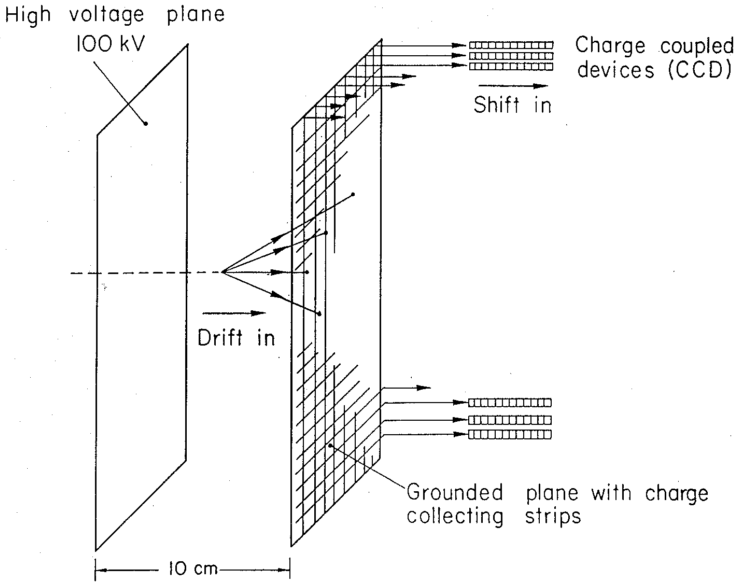
\includegraphics[width=10cm]{RubbiaLArTPC.png}
  \caption[First LArTPC detector, Rubbia (1977)]{The LArTPC detector proposed by Carlo Rubbia in 1977 \cite{Rubbia1977}.}
  \label{fig:RubbiaLArTPC}
\end{figure}

Constructing and operating such a detector was beyond the technology of the time, and is still being understood today.  The operation of a LArTPC detector is described in Section~\ref{sec:LArTPCOperation} and the associated challenges are the subject of Section~\ref{sec:LArTPCChallenges}.

%----------------------------------------------------------------------------------------------------------------------------------------------------------------------------
\subsection{LAr TPC Operation}\label{sec:LArTPCOperation}

A LArTPC typically consists of one or more anodes and cathodes at either end of an active drift region.  An ionising particle passing through a LArTPC causes electrons to become free from argon atoms and, in the presence of a field, drift towards an anode where they are read out.

There are two differing designs of LArTPC: single-phase and dual-phase.  In a single-phase design, only argon in a liquid state is utilised and the entire detector, including target medium, propagation, readout and signal processing take place within the liquid.  In contrast, a dual-phase design would employ a layer of gaseous argon above the liquid, through which the drift electrons are extracted before readout.  This has the primary advantage of amplification of signal due to electron avalanches in an electric field in the gas and therefore a lower detection threshold but also results in a larger fiducial volume with the absence of dead regions in the LAr volume.

The readout consists of multiple wire planes with different orientations to facilitate the reconstruction.  The wires are either `induction' wires, which allow the electrons to deposit charge but continue past, or `collection' wires, on which the electric field lines end and all the charge on the electron is collected.  Each wire plane is therefore held at a different `bias voltage' to prevent any field lines ending on the induction wire, thus creating local electric fields which promote the continuing forward motion of the electrons.  The signal seen is therefore dependent on the type of wire plane; a bipolar pulse on an induction plane wire and unipolar on a collection plane wire.  It is also common, though not essential, to make use of a `grid plane' upstream of the signal planes in order to shield them from the electron charge until the drift electrons are close.  Without such a plane, the bipolar pulse would be highly asymmetric, though would still have zero integral.  It also makes changing the drift voltage (controlling the electric field) slightly easier as the signal planes are somewhat shielded from its effects.  MicroBooNE does not operate with a grid plane and, although the 35~ton and the DUNE reference design make use of a grid plane, it is uncertain whether the benefit outweighs the cost for a huge LArTPC detector such as the DUNE far detector.  There are alternative readout possibilities to this typical design which have been suggested but, given the scale of future LArTPCs, it is highly unlikely a viable solution which delivers superior readout at a comparable cost will be found.

Upon ionisation, an electron has a certain probability (around 60\%) of recombining before the field can separate it from its ion.  Whilst this compromises the signal observed, it is accompanied by a flash of scintillation light which may be detected and used to assign an `event time' to the interaction, known as T0.  Without this information, it would be impossible to place an absolute time scale on the event and result in an unresolved coordinate along the drift direction.  The magnitude of the applied electric field must be chosen to balance these two effects; a larger field would result in less recombination and therefore compromise the scintillation light while a smaller field would have consequences on the signal received at the wire planes.  Figure~\ref{fig:ElectricFieldScintillationIonisation} demonstrates this and justifies the field value of 500~V/cm which is often chosen in current LAr neutrino experiments.

\begin{figure}
  \centering
  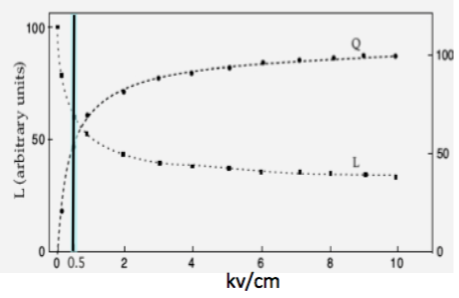
\includegraphics[width=12cm]{ElectricFieldScintillationIonisation.png}
  \caption[Effect of electric field on luminosity of ionisation electrons and scintillation light in a LArTPC.]{Demonstration of the competing effect the electric field has on the luminosity of the ionisation electrons and scintillation light arriving at the detector readout.  Since both are essential in reconstructing the complete interactions, a balance must be found. [PLACEHOLDER IMAGE].}
  \label{fig:ElectricFieldScintillationIonisation}
\end{figure}

The basic operational principles of a LArTPC is demonstrated in Figure~\ref{fig:LArTPCOperation}.  The specifics of how the ionisation charge and the scintillation light is collected and processed is experiment-specific and will be discussed in the context of DUNE in Chapter \ref{chap:DUNE} and the 35~ton experiment in Chapter \ref{chap:35ton}.  This information is all that is required to fully understand and analyse the interactions occurring in the detector; methods used to reconstruct particles and interactions in LAr will be the subject of Chapter \ref{chap:LArTPCReconstruction}.

\begin{figure}[p]
  \centering
  \begin{subfigure}[t]{0.48\linewidth}
    \centering
    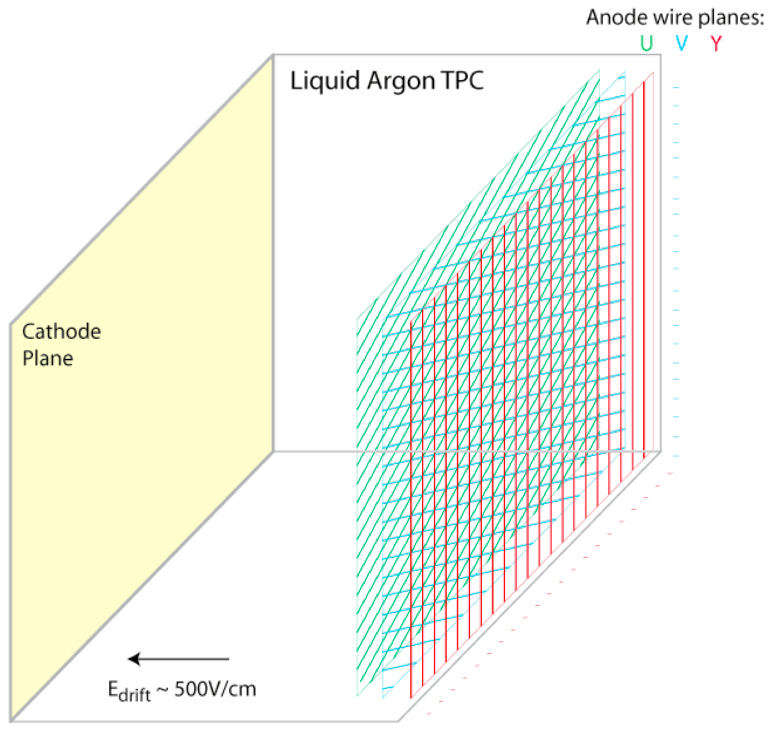
\includegraphics[width=0.98\textwidth]{LArTPCOperation1.png}
    \caption{Typical LArTPC with one cathode (left) and three read out anode planes (right) (two induction, U and V, and one collection, Y), setting up an electric field.  The central region is filled with liquid argon.}
    \label{fig:LArTPCOperation1}
  \end{subfigure}
  \hfill
  \begin{subfigure}[t]{0.48\linewidth}
    \centering
    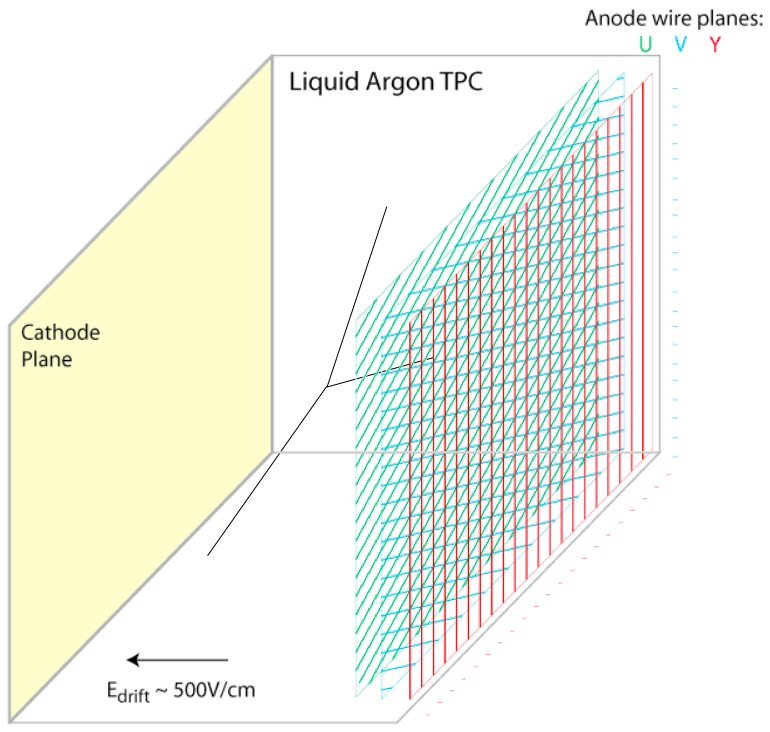
\includegraphics[width=0.98\textwidth]{LArTPCOperation2.png}
    \caption{An ionising particle enters the detector and liberates electrons from the medium, which then drift towards the anode planes.}
    \label{fig:LArTPCOperation2}
  \end{subfigure}
  \hfill
    \begin{subfigure}[t]{0.48\linewidth}
    \centering
    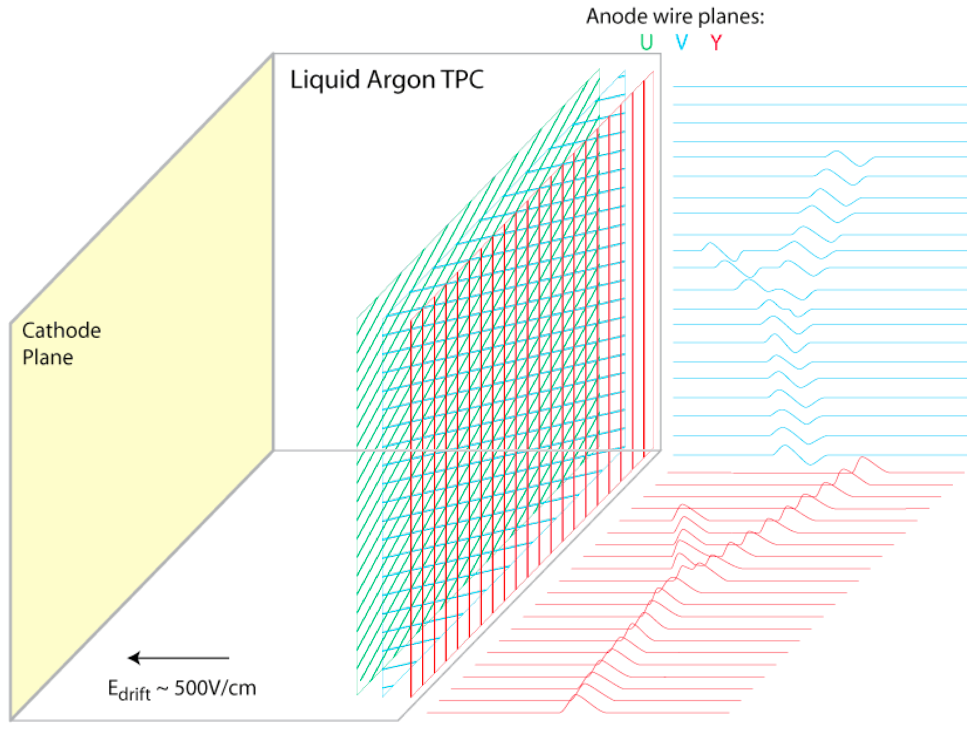
\includegraphics[width=0.98\textwidth]{LArTPCOperation3.png}
    \caption{As the electrons drift through, charge is induced on the first two wire planes and collected on the final one.  Due to the differing orientations of the wires between planes, three complementary views of the interaction are provided (two are shown).}
    \label{fig:LArTPCOperation3}
  \end{subfigure}
  \hfill
  \begin{subfigure}[t]{0.48\linewidth}
    \centering
    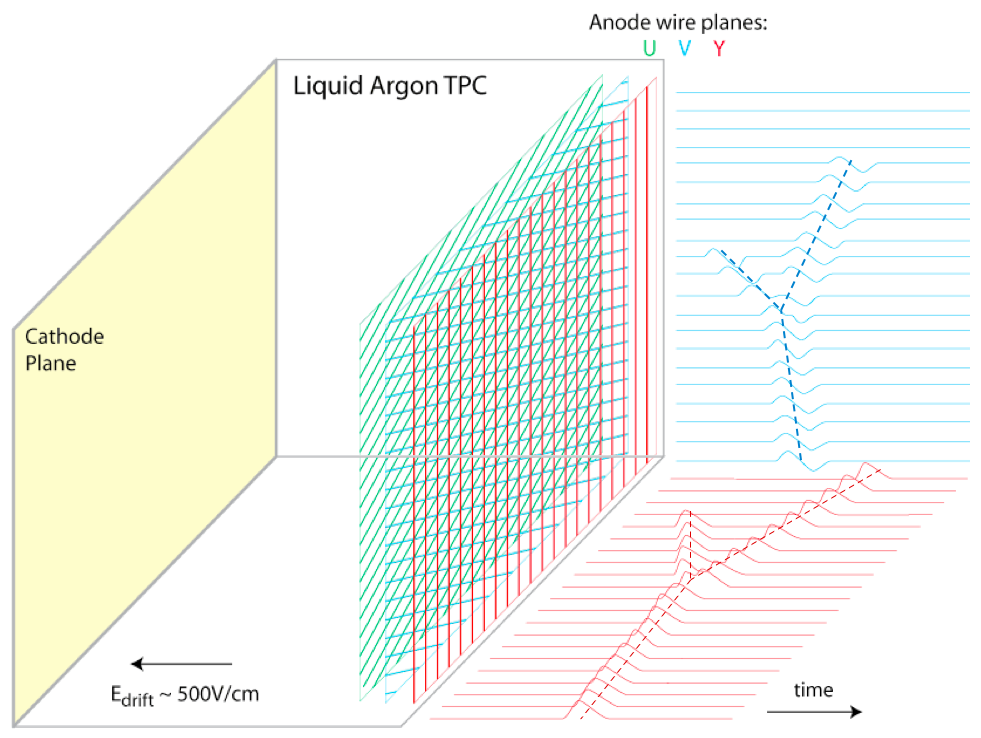
\includegraphics[width=0.98\textwidth]{LArTPCOperation4.png}
    \caption{By combining the two dimensional information provided by the anode planes with the drift time information, the original particle tracks can be inferred.}
    \label{fig:LArTPCOperation4}
  \end{subfigure}
  \caption[Schematic demonstrating the basic operational principles of a LArTPC.]{Schematic demonstrating the basic operational principles of a LArTPC.  The images are stills taken from an illustration created by Bo Yu (BNL) {\color{red}(do I need to cite this?  It's a very common slide and I can't actually find a Bo Yu talk with it in... everyone just puts his name on the slide!)}.}
  \label{fig:LArTPCOperation}
\end{figure}

%----------------------------------------------------------------------------------------------------------------------------------------------------------------------------
\subsection{LArTPC Challenges}\label{sec:LArTPCChallenges}

There is no doubt of the promise of LArTPCs for the future of neutrino physics but with such expectation comes many challenges.  This will be elaborated upon in more detail when discussing the 35~ton run in Section~\ref{sec:35tonPhaseII} but will be briefly mentioned here for completeness.

Given the drift fields required, and the necessary distances, the associated high voltage on the cathode must be on the order of $\sim$100~kV.  This presents engineering challenges related to the feedthrough and cryostat design but also can lead to dielectric breakdown of the liquid nearby such huge voltages.  The properties of LAr and the design implications must be very well understood to ensure this does not endanger the quality of the detector medium.

The presence of electro-negative impurities in the argon can capture drift electrons as they travel towards the anode planes and hinder the signal observed.  The probability of this recombination is referred to as the `electron lifetime' and is directly affected by the maintained purity of the argon.  DUNE expects a contamination no greater than 100 ppt O$_2$ and 20 ppm N$_2$ (to also ensure sufficient light yield) \cite{DUNECDR4}.  This necessitates a purification system to remove impurities and requires the constant recirculation of the liquid through it.  A liquifier is also necessary to recondense any boiled-off gases at the surface.

Along with the possibility of lost signal through finite electron lifetimes, the electrons may also undergo interactions and drift off course either transversely or longitudinally.  This `diffusion' affects the location and size of the observed signal so must also be well understood.

With so much resting on the success of the DUNE experiment, and considering all these effects which must be understood, prototyping is essential.  The 35~ton prototype was constructed as an attempt to better understand LArTPCs and is the subject of Chapter \ref{chap:35ton}.

%----------------------------------------------------------------------------------------------------------------------------------------------------------------------------
\section{Overview of DUNE}\label{sec:DUNEOverview}

The outstanding questions in neutrino physics discussed in Section~\ref{sec:NeutrinoPhysicsStatus}, namely the resolution of the mass hierarchy, the determination of the CP-violating phase $\delta_{\textnormal{CP}}$, the measurement of the octant of $\theta_{23}$ and precision calculations of all the mixing angles, motivate the need for next generation experiments.  The DUNE experiment will make decisive contributions to each of these areas; it will also search for nucleon decay with the ability to set world-leading proton lifetime limits and make detailed, unique measurements of the $\nu_e$ flux from a core-collapse supernovae within our galaxy should one occur during the experiment.  Along with this, DUNE will be used to look for Beyond Standard Model physics (such as non-standard interaction and sterile neutrinos), signatures of dark matter and, utilising the capable near detector, measurements of a range of neutrino cross-sections and nuclear effects including final state interactions.

The chosen technology for the DUNE far detector, in order to maximise sensitivity to all these factors, is a LArTPC, introduced and described in Section~\ref{sec:LArTPC}.  The detector will contain four modules, each comprised of 10~kt fiducial LAr and separate data acquisition and readout systems.  The beam will be provided by Fermilab as part of its PIP-II program \cite{PIPII2013} and will be wide band, enabling the study of a range of neutrino energies.  This facilitates a study of multiple oscillation peaks, essentially due to differing $L/E$ ratios, and is relevant when considering the effects of an unknown CP-violating phase and unresolved mass hierarchy.  Since the impact of both of these uncertainties is apparent as an asymmetry between neutrinos and antineutrinos (Equation \ref{eq:NeutrinoAntineutrinoAsymmetry}), there is an implicit degeneracy which must be resolved to ensure both phenomena are correctly determined.  Having access to multiple oscillation peaks means this may be dealt with in a single experiment, as demonstrated in Figure~\ref{fig:TwoPeakAmbiguity} \cite{Huber2011}.

\begin{figure}
  \centering
  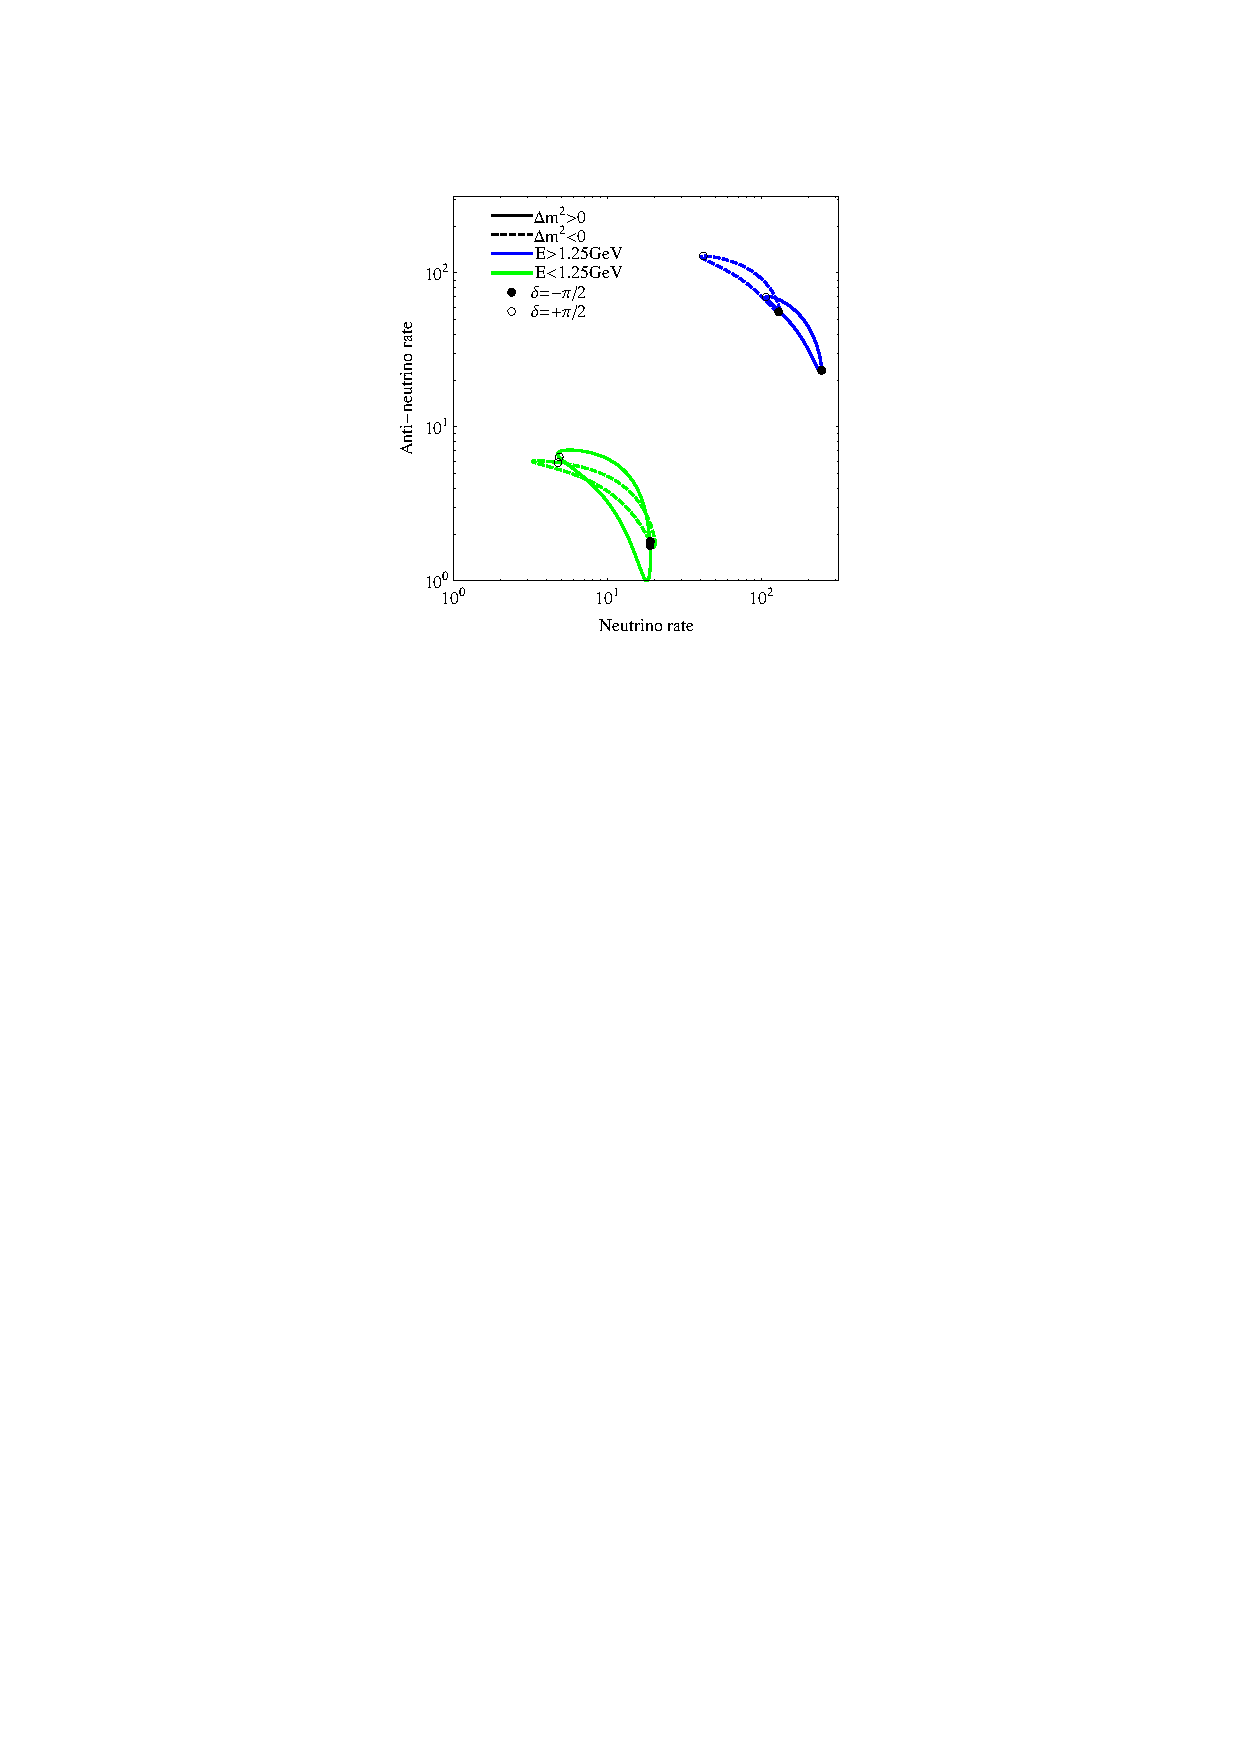
\includegraphics[width=10cm]{TwoPeakAmbiguity.pdf}
  \caption[Demonstration of how having access to multiple oscillation maxima facilitates measurements of both the neutrino mass hierarchy and leptonic CP violation using the same experiment.]{Demonstration of how having access to multiple oscillation maxima facilitates measurements of both the neutrino mass hierarchy and leptonic CP violation using the same experiment.  In the plot, $\theta_{13}$ is held constant and the rates are determined by the number of neutrino and antineutrino events respectively.  Assuming a baseline of 1300~km, as for DUNE, the first oscillation maximum is at $E_{\nu}=2.5$~GeV and the second is at $E_{\nu}=0.84$~GeV.  The banana-shaped distributions are obtained as the value of $\delta_{CP}$ is varied from $-\pi$ to $\pi$.  There is good separation between the distributions associated with each hierarchy at the first maximum whereas at the second maximum this is degenerate and the rates are similar for a given value of $\delta_{CP}$ regardless of the hierarchy.  It can be seen how complimentary measurements at each maxima can be used to make unambiguous measurements of both the mass hierarchy and of CP violation with the same experiment.  Taken from \cite{Huber2011}.}
  \label{fig:TwoPeakAmbiguity}
\end{figure}

DUNE was officially formed in early 2015 following the dissolution and merging of two leading next generation long-baseline experiments: the Long Baseline Neutrino Experiment (LBNE) in the U.S. \cite{LBNECDR1,LBNECDR3,LBNECDR4a} and the Large Apparatus for Grand Unification, Neutrino Astrophysics, and Long Baseline Neutrino Oscillations (LAGUNA-LBNO) in Europe \cite{LAGUNA-LBNO2015}.  Given the scale of these projects, it was decided in 2014 that efforts should be focussed on one flagship experiment utilising the expertise of as many experts in neutrino physics and LArTPC technology as possible \cite{P52014}.  The benchmark DUNE design is very similar to that of the former LBNE experiment, which also made use of an upgraded Fermilab neutrino beam and a large LArTPC at SURF, and gained the understanding of dual-phase LArTPC detectors developed by LAGUNA-LBNO.  It is likely that at least one of the four DUNE detector modules will be a dual-phase LArTPC.

The experiment will be facilitated by the Long Baseline Neutrino Facility (LBNF), which will oversee the technical side of the project and ensure the DUNE experiment can function as desired.  The relationship between the LBNF and the DUNE projects is based on the model used at CERN to manage the Large Hadron Collider (LHC) and each of the experiments which use it.  LBNF has its own management structure and operates separately from DUNE, though the two projects work closely together.  It is supported mainly via the Department of Energy in the U.S. whereas DUNE is internationally funded.  The DUNE collaboration is responsible for defining the scientific goals of the experiment and the corresponding technical requirements.  Using these, LBNF will design and construct all technical facilities, such as the beam upgrade, the facilities for the near detectors at Fermilab and the excavation and outfitting of the large caverns for the far detectors underground at SURF along the required infrastructure to support the construction of the cryostats and the associated cryogenic systems.  DUNE will provide the four massive LArTPCs and the near detector systems, to be constructed at the sites supplied by LBNF.  These will be discussed further in Section~\ref{sec:DUNEExperiment}.  During the lifetime of the experiment, LBNF is responsible for the maintaining and operation of all the facilities whilst DUNE will commission and operate the detectors.  The scientific research program conducted with the collected data is the duty of the DUNE collaboration and will be explored in Section~\ref{sec:DUNEPhysics}.

Given the scale of the projects, work is already underway.  Construction at the far detector site starts this year, with installation of the first detector module due to commence in 2021.  The start of the DUNE experiment will then correspond to the completion of this module, scheduled in 2024.  The PIP-II upgraded 1.2~MW beam will be ready in 2025 and will signify the commencement of beam data taking.  Subsequent detector modules will be added as soon as is feasible thereafter, increasing the fiducial volume up to the target mass of 40~kt.  Further beam upgrades, up to 2.4~MW (PIP-III) are envisaged beyond this to bring the experiment up to full power and maximise the physics capability of the project.  The timescales of both LBNF and DUNE, along with all the essential research which must be conducted as the plans progress, is the subject of Section~\ref{sec:RoadToDUNE}.

%----------------------------------------------------------------------------------------------------------------------------------------------------------------------------
\section{Experimental Details}\label{sec:DUNEExperiment}

The design of the DUNE experiment is driven by the physics ambition of the project and all specific experimental details are motivated by the science DUNE wishes to study.  This section will briefly report on the current understanding of how DUNE will be planned.  It should be noted that whilst the important defining features of the design will endure it is likely, given the timescales of the project, particular details will charge for the final proposal.

The plans for the beam will be overviewed in Section~\ref{sec:DUNEBeam} before the present considerations for the far and near detectors are presented in Sections~\ref{sec:FarDetector} and~\ref{sec:NearDetector}.

%----------------------------------------------------------------------------------------------------------------------------------------------------------------------------
\subsection{Beam}\label{sec:DUNEBeam}

The beam is required to be wide band to facilitate access to the first two oscillation maxima (at 1300~km, 2.4~GeV and 0.8~GeV).  It is a conventional, horn-focussed, sign selected neutrino beam and is detailed in Figure~\ref{fig:DUNEBeam}.

\begin{figure}
  \centering
  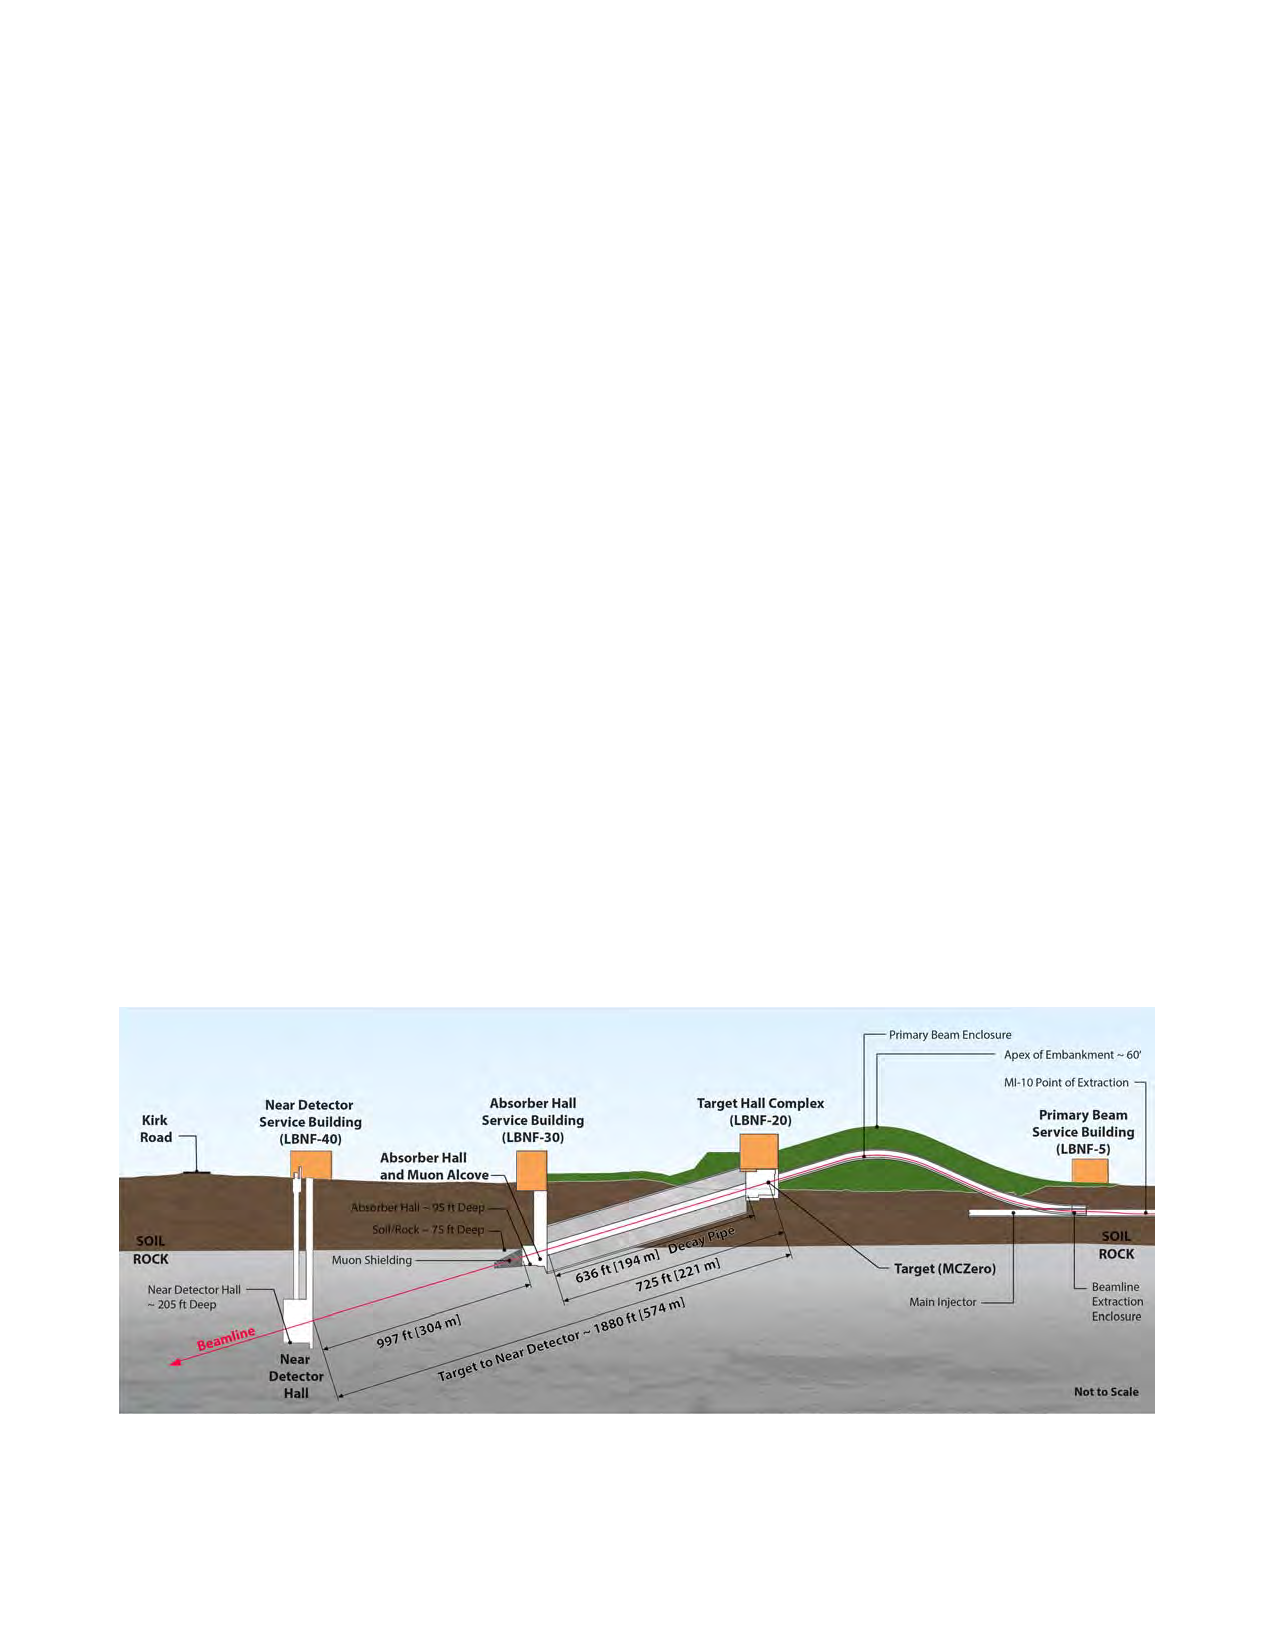
\includegraphics[width=14cm]{DUNEBeam.pdf}
  \caption{Longitudinal section of the LBNF beamline facility at Fermilab \cite{DUNECDR3}.}
  \label{fig:DUNEBeam}
\end{figure}

A proton beam (60-120~GeV) is extracted from the Fermilab Main Injector, transported through a man-made embankment and bent downwards to establish the final trajectory towards the far detector.  The beam is incident on a target to produce secondary mesons which are subsequently focussed into a decay pipe by magnetic horns where they decay into muons and neutrinos.  The polarity of the horns used determines whether or not the beam is neutrino or antineutrino dominated.  At the end of the decay pipe, the muons and any residual hadrons are stopped to produce a beam of neutrinos, tuned with energies between 0.5~GeV and 5~GeV.  The fluxes of different neutrino species present in the beam in both neutrino- and antineutrino-running modes are shown in Figure~\ref{fig:DUNEBeamFluxes}.  The target is based on the design used in the Fermilab NuMI (Neutrinos from Main Injector) beam, in operation since 2005, and consists of a graphite core with dual titanium water lines to dissipate heat, encased in a titanium containment tube.

\begin{figure}
  \centering
  \begin{subfigure}[t]{0.48\linewidth}
    \centering
    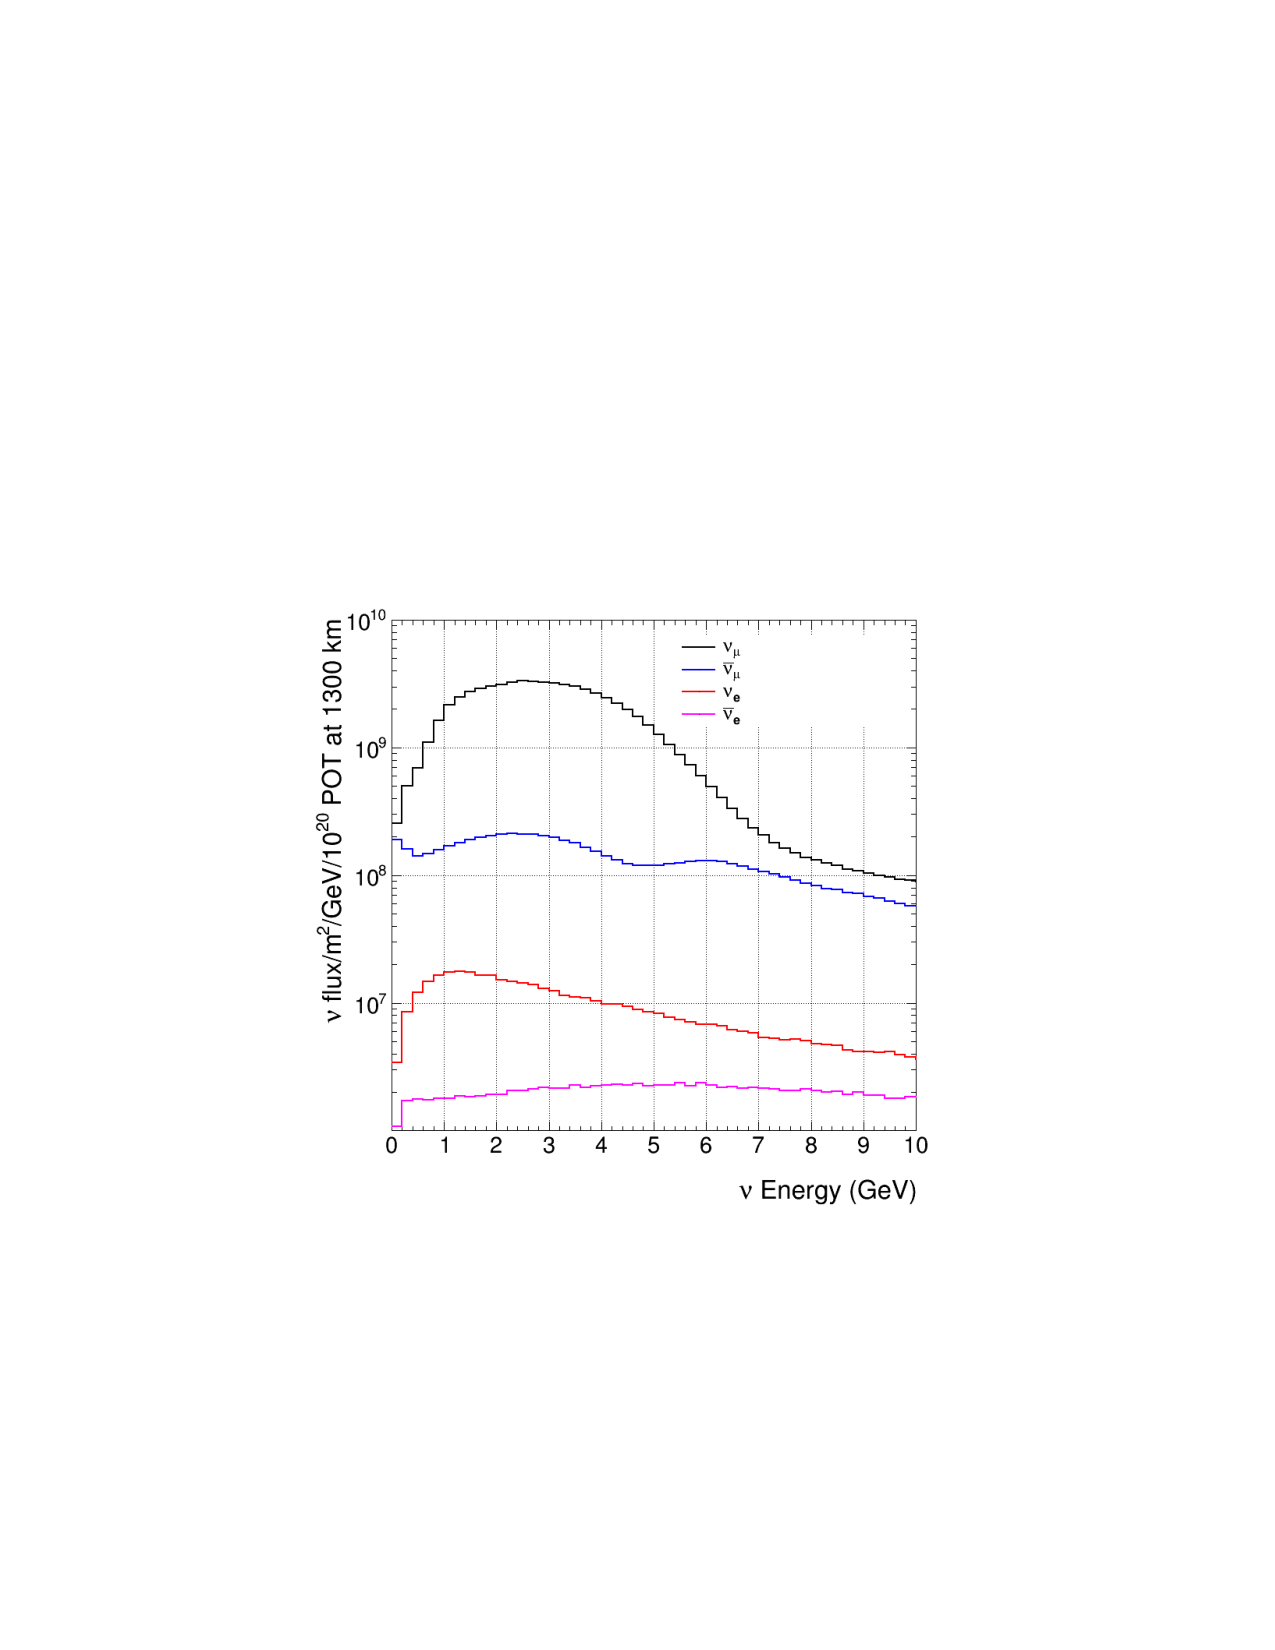
\includegraphics[width=0.98\textwidth]{DUNEBeamFluxesNeutrino.pdf}
    \caption{Neutrino running.}
    \label{fig:DUNEBeamFluxesNeutrino}
  \end{subfigure}
  \hfill
  \begin{subfigure}[t]{0.48\linewidth}
    \centering
    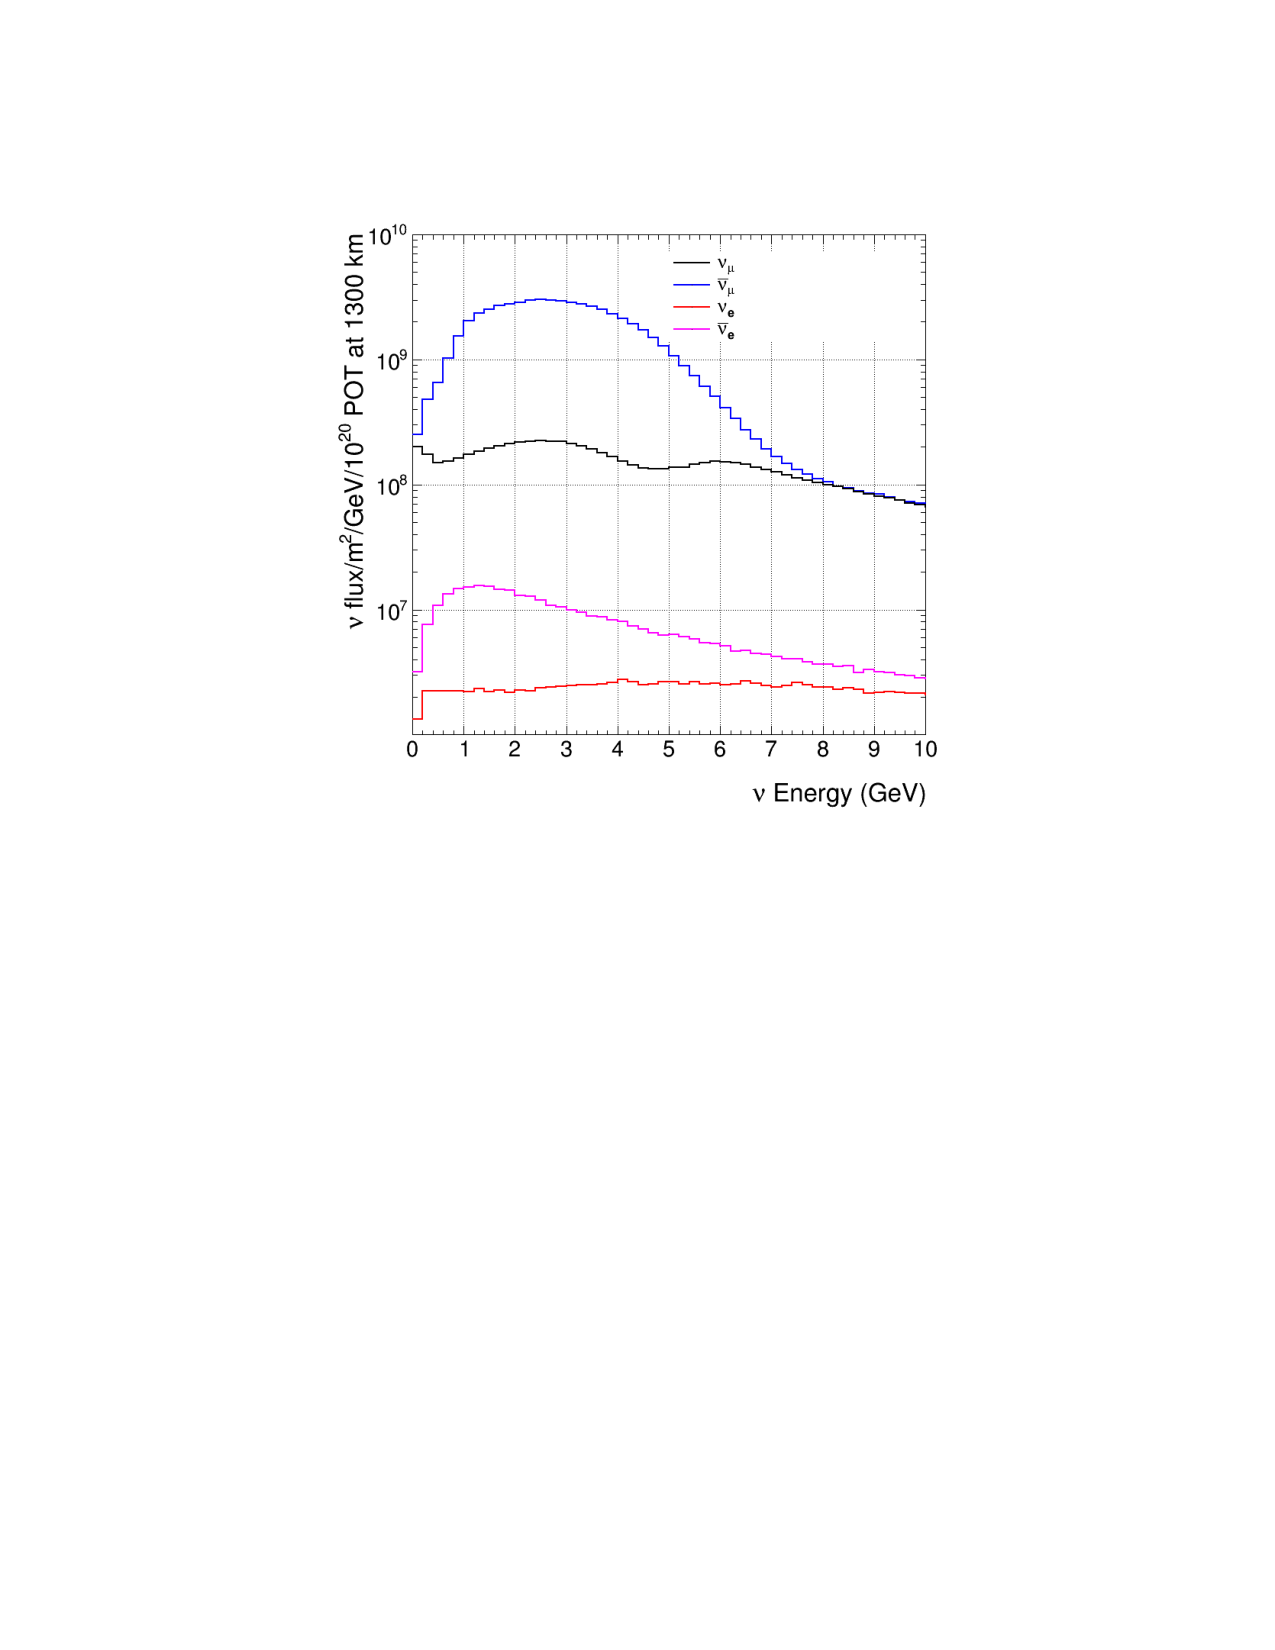
\includegraphics[width=0.98\textwidth]{DUNEBeamFluxesAntiNeutrino.pdf}
    \caption{Antineutrino running.}
    \label{fig:DUNEBeamFluxesAntiNeutrino}
  \end{subfigure}
  \caption[The fluxes of the different neutrino flavour components of the DUNE beam in neutrino and antineutrino running mode.]{The fluxes of the different neutrino flavour components of the DUNE beam in neutrino and antineutrino running mode \cite{DUNECDR3}.}
  \label{fig:DUNEBeamFluxes}
\end{figure}

The current beam design has been evolving since 2012 when it was first conceived for the LBNE experiment.  Many potential optimisations have been identified and some are now part of the reference design; others are still in the process of evaluation.  In the sensitivities presented in Section~\ref{sec:DUNEPhysics}, two beam configurations are referred to: reference and optimised.  The optimised design pertains to such ongoing considerations envisioned to improve performance, for example in flux at the first and especially the second oscillation maximum and in the reduction of wrong-sign neutrino backgrounds.  The improvements are foreseen to come from an thorough assessment of the target-horn system and will influence the reference design as the beam plans become more mature.

%----------------------------------------------------------------------------------------------------------------------------------------------------------------------------
\subsection{Far Detector}\label{sec:FarDetector}

There are two potential designs for a far detector LArTPC utilising either single-phase or dual-phase LArTPCs.  Both are under consideration in the upcoming ProtoDUNE prototypes (described in Section~\ref{sec:RoadToDUNE}) and final decisions will be taken upon their completion and on reflection on the status of the technology.  The first module will certainly employ a single-phase design with future instalments potentially either.  The design of the cryostats, demonstrated in Figure~\ref{fig:FDCryostats}, is such that only minor modifications would be required when switching between technologies.  Each cryostat will hold a fiducial/active/total LAr mass of 10.0/13.3/17.1~kt.

\begin{figure}
  \centering
  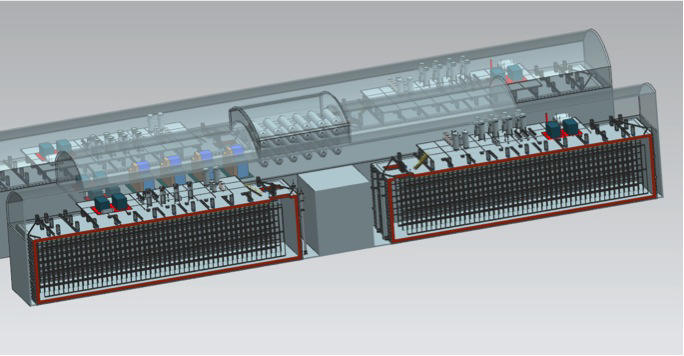
\includegraphics[width=12cm]{FDCryostats.png}
  \caption[The layout of the four cryostats underground at SURF comprising the DUNE far detector.]{The layout of the four cryostats underground at SURF comprising the DUNE far detector \cite{DUNECDR4}.  The detectors occupying the cryostats here are of the single-phase design, however they can also be used to accommodate detectors utilising dual-phase technology.}
  \label{fig:FDCryostats}
\end{figure}

The basic features of each detector design will be overviewed in the following sections.  As the first detector will be single-phase, and the work detailed in this thesis pertains solely to this detector design, a much greater emphasis will be placed on this design choice in the proceeding discussions.

%----------------------------------------------------------------------------------------------------------------------------------------------------------------------------
\subsubsection{Single-Phase}\label{sec:DUNESinglePhase}

The layout of the single-phase DUNE detector design is shown in Figure~\ref{fig:DUNEFarDetectorDesign}.  The modular form of the detector ensures it is flexible and scalable and facilitates the transportation and assembly of component parts.  The detector units are named Anode Plane Assemblies (APAs) and Cathode Plane Assemblies (CPA) and, as their names suggest, carry the required voltages necessary to establish the electric field.  The active volume is 12~m high, 14.5~m wide and 58~m long in the beam direction, with the APAs and CPAs placed such that their planes are parallel to the beam.  Each APA is 2.3~m wide and 6~m high, requiring them to be stacked two high and 25 long to instrument the required volume.  The CPAs have the same width but half the height so must be stacked four high and, given the drift distance of 3.6~m, carry a voltage of $-180$~V in order to provide the required field of 500~V/cm.  Each module therefore contains 150~APAs and 200~CPAs, surrounded on its open sides by a field cage.  The entire TPC is suspended from the ceiling of the cryostat on rails.

\begin{figure}
  \centering
  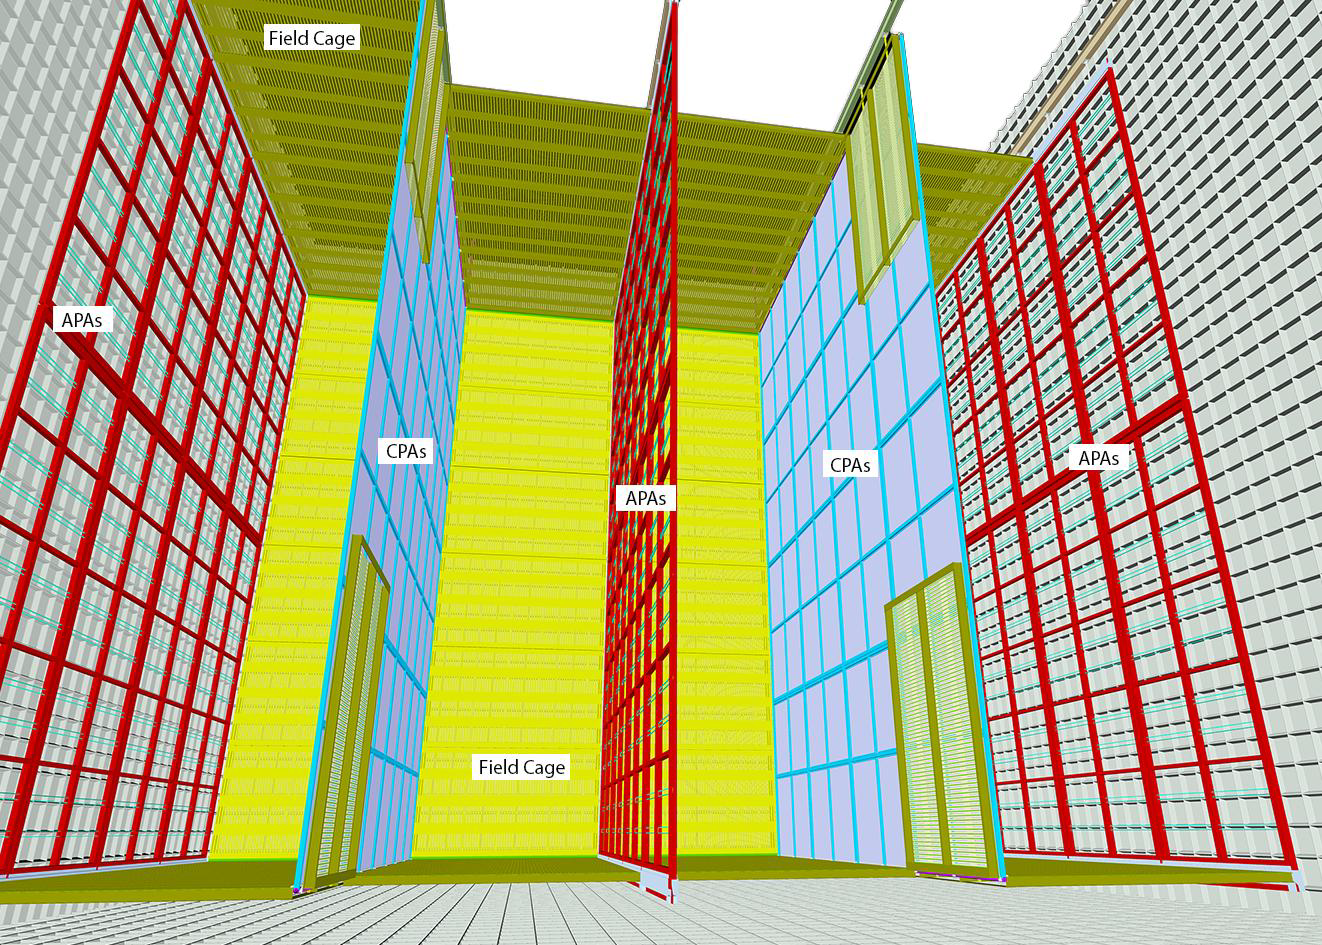
\includegraphics[width=14cm]{DUNEFarDetectorDesign.png}
  \caption[The basic design of a single-phase DUNE far detector module.]{The basic design of a single-phase DUNE far detector module \cite{DUNECDR4}.  The beam direction is into the page and the electric field, provided by the Anode Plane Assemblies (APAs) and Cathode Plane Assemblies (CPAs), is perpendicular to this across the page.}
  \label{fig:DUNEFarDetectorDesign}
\end{figure}

\begin{figure}
  \centering
  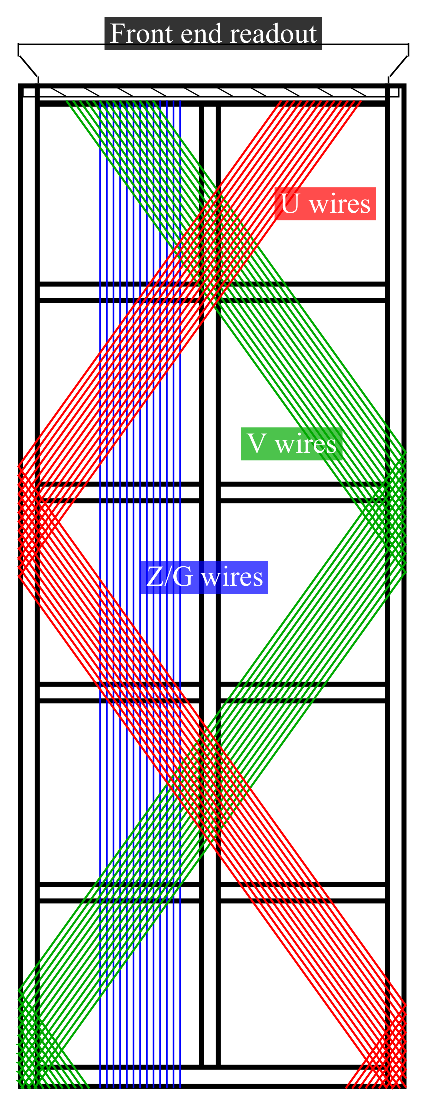
\includegraphics[width=6cm]{FarDetectorAPA.eps}
  \caption[Design of a DUNE far detector Anode Plane Assembly (APA).]{Design of a DUNE far detector Anode Plane Assembly (APA).  The three instrumented planes, collection (Z) and two inductions (U and V), are shown in blue, red and green respectively.  The grid plane is not shown but is parallel to the collection wires.  The induction wires are wrapped around the frame and make angles of $\pm35.7^{\circ}$ to the vertical, chosen so that each wire segment crosses each collection channel no more than once.  This ensures there is no ambiguity in the side of the APA the charge arrived at.}
  \label{fig:DUNEFarDetectorAPA}
\end{figure}

The basic design of an APA is demonstrated in Figure~\ref{fig:DUNEFarDetectorAPA}.  Each comprises four sets of wire planes; from the outside in: a grid plane (G), two induction views (U and V) and a collection plane (Z).  The APAs are designed to maximise active detector region and are therefore stacked as closely together as possible and read out charge from multiple drift regions simultaneously.  This requires all readout be positioned at the top (or bottom of lower APAs) of the frame and use of a wrapped wire approach for the induction wires, since these must be fixed at an angle.  This wrapping also carries the added benefit of reducing the number of channels required since a wire from the U plane on one side of an APA is part of the V plane on the opposite side.  The collection and grid wires are both vertical, necessitating a set for each face of an APA.  A single wire reading out multiple drift regions concurrently potentially leads to an ambiguity in the particular wire segment at which the charge arrived.  This is broken in one of two ways; either the wires in the U and V planes are placed at slightly different angles, reducing the number of triple crossing points with a given collection wire, or the angle of the induction plane wires is chosen such that each wire segment intersects no more than one collection wire.  The former is prototyped in the 35~ton experiment whilst the current plan for the DUNE far detector is to opt for the latter.  An angle of $\pm35.7^{\circ}$ ensures this is the case, demonstrated in Figure~\ref{fig:DUNEFarDetectorAPA}.  A grounded mesh, with good optical transparency, is fixed to the face of the APA frame behind each collection plane to ensure a uniform electric field in the region inside the APA, between the two sets of biased collection wires and the grounded frame.

The front-end electronics are mounted on the APAs and function within the cryostat; it is for this reason they are referred to as `cold electronics'.  They are implemented as two successive ASIC chips, the first providing amplification and signal shaping and the second the digitisation of the signal.  Early versions of these chips were utilised in the 35~ton experiment for front-end readout. {\color{red} Note to me: could put picture of signal shaping here if it appears necessary as I write about the 35ton stuff...}

The external triggering in the DUNE far detector relies on detecting the scintillation light from immediate recombination of ionisation electrons with the argon ions.  This requires dedicated photon detectors which may detect this light with suitable efficacy.  At a field of 500~V/cm, the photon yield is around 20,000 per MeV at wavelengths of 128~nm.  The current reference design, depicted in Figure~\ref{fig:DUNEPhotonDetectors}, involves placing light-guides, containing wavelength shifter, at the centre of each APA frames and using SiPMs for readout.  There will be 10 per APA, to be inserted after wire wrapping, with dimensions 2.2~m long, 83~mm wide and 6~mm thick.

\begin{figure}
  \centering
  \begin{subfigure}[t]{0.48\linewidth}
    \centering
    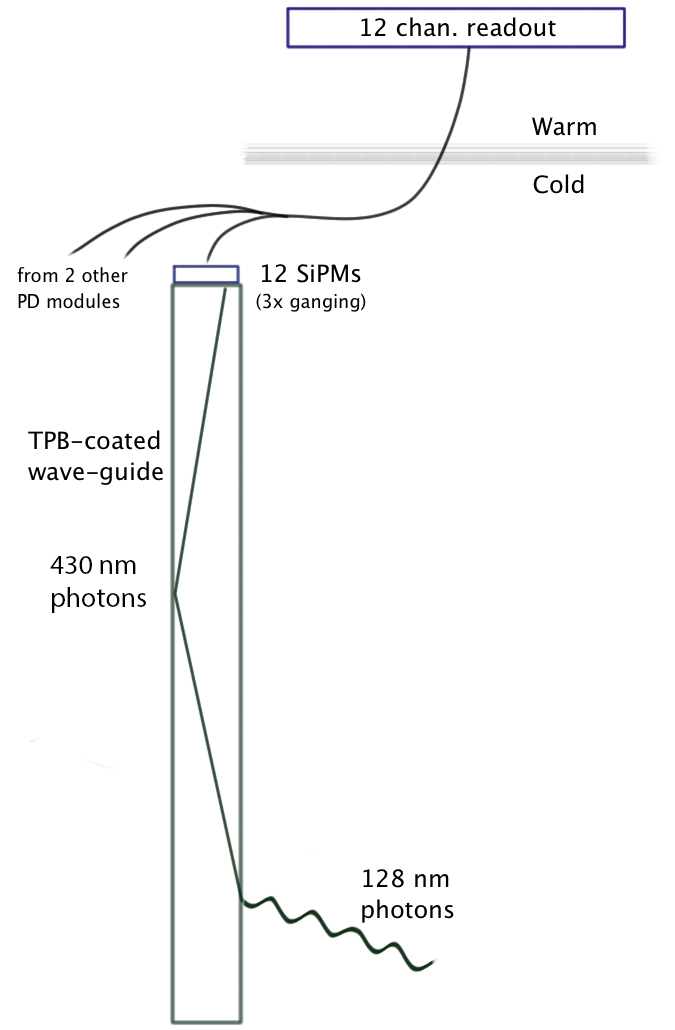
\includegraphics[height=6cm]{DUNEPhotonDetectors.png}
    \caption{Photon detector design.}
    \label{fig:DUNEPhotonDetectorsBar}
  \end{subfigure}
  \hfill
  \begin{subfigure}[t]{0.48\linewidth}
    \centering
    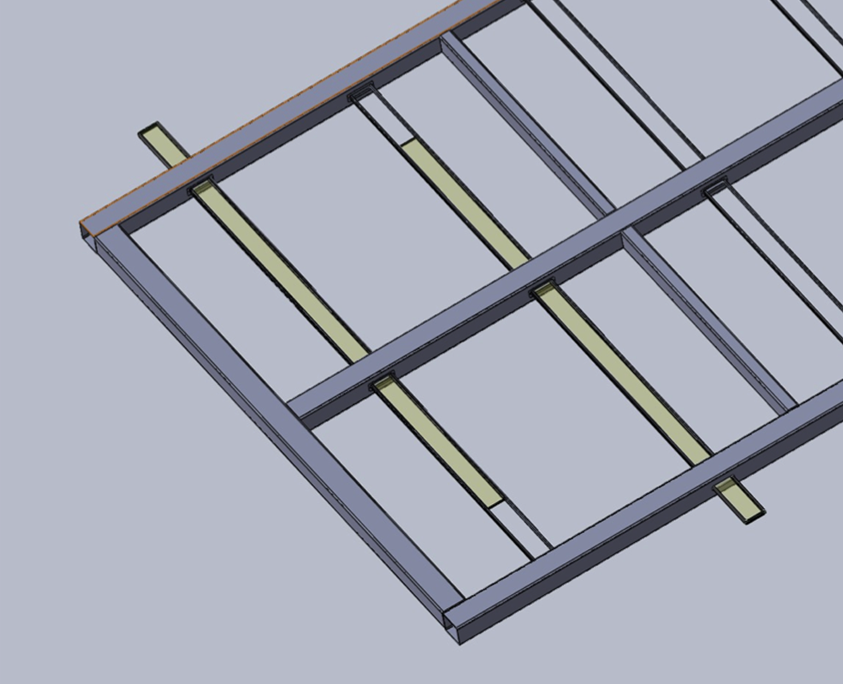
\includegraphics[height=6cm]{DUNEPhotonDetectorsAPA.png}
    \caption{Photon detectors in an APA.}
    \label{fig:DUNEPhotonDetectorsAPA}
  \end{subfigure}
  \caption[The design of the photon detectors for the DUNE far detector.]{The design of the photon detectors for the DUNE far detector \cite{DUNECDR4}.  The basic design of each bar is shown in Figure~\ref{fig:DUNEPhotonDetectorsBar} and their positioning within an APA is shown in Figure~\ref{fig:DUNEPhotonDetectorsAPA}.}
  \label{fig:DUNEPhotonDetectors}
\end{figure}

Overall, optimisation of this detector design involves considerations of the physics reach as well as the associated cost, schedule and risks.  Relevant decisions concern the spacing between the readout wires (`pitch'), which directly affects the detector resolution; the spacing between the wire planes, affecting the shape of the field; the wire angle, necessary for reconstruction but with possible ambiguities; the wire length, affecting the noise levels observed; and the maximum drift length, which influences the size of signal observed.  Each has been optimised to ensure the physics goals are reached while reducing as much as possible the cost of the detectors.

%----------------------------------------------------------------------------------------------------------------------------------------------------------------------------
\subsubsection{Dual-Phase}\label{sec:DUNEDualPhase}

The DUNE dual-phase LArTPC design differs from its single-phase counterpart in that the cathode is placed at the bottom of the cryostat, with the anode readout at the top (above the gas layer), demonstrated in Figure~\ref{fig:DUNEDualPhase}.  This sets up a field in the vertical direction and results in upwards electron drift.  The detector is a single volume, 60~m long, 12~m wide and 12~m high.  Due to the gain provided by the gas phase, the required argon purity is equivalent to the single-phase detector despite the electron drift being more than three times greater.  Each module additionally contains 180 PMTs (1 per 4~m$^2$), located underneath the cathode.

\begin{figure}
  \centering
  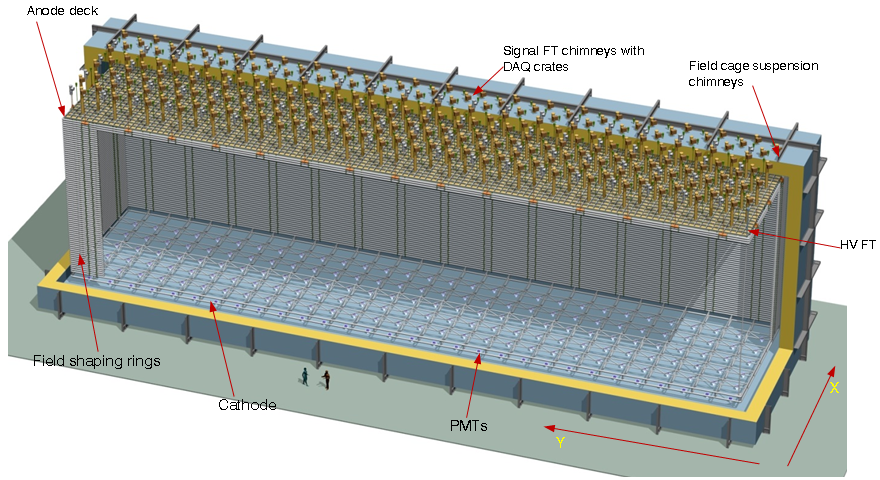
\includegraphics[width=14cm]{DUNEDualPhase.png}
  \caption[The DUNE dual-phase detector (partially open).]{The DUNE dual-phase detector (partially open) \cite{DUNECDR4}.  The cathode is at the bottom of the cryostat, with the PMTs responsible for detecting the scintillation light beneath.  The anode is at the top, resulting in upwards electron drift, above a layer of gaseous argon present to introduce a gain in the collected signal.}
  \label{fig:DUNEDualPhase}
\end{figure}

The amplification uses Large Electron Multipliers (LEMs): printed circuit boards with electrodes at the top and bottom surfaces across which a potential difference is applied.  The data collection is performed by modules named Charge Readout Planes (CRPs), each containing many LEM/anode sandwiches and two independent, orthogonal readout views.  The basic operation, including the electric fields at each point in the electron extraction, amplification and readout, is demonstrated in Figure~\ref{fig:DUNEDualPhaseCRP}.  As with the single-phase design, the nominal drift field in the liquid is 0.5~kV/cm.  The electrons are extracted from the liquid with 100\% efficiency using a 2~kV/cm field and are amplified in a field on the order of 30~kV/cm, providing a gain between 20-100.  The readout utilises two perpendicular collection planes at the same level which allow full 3D reconstruction when combined with the location in the drift direction from photon detector information.  Each CRP has dimensions $3\times3$~m$^2$ (containing 36 ($0.5\times0.5$~m$^2$) LEM/anode sandwiches) and each module requires 80 such instruments to read out the active volume.

\begin{figure}
  \centering
  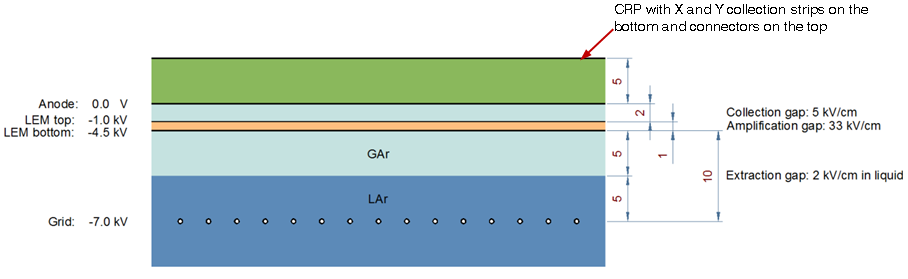
\includegraphics[width=14cm]{DUNEDualPhaseCRP.png}
  \caption[The extraction, amplification and readout of the ionisation electrons through the gaseous argon phase in the DUNE dual-phase LArTPC design.]{The extraction, amplification and readout of the ionisation electrons through the gaseous argon phase in the DUNE dual-phase LArTPC design \cite{DUNECDR4}.  The voltages at each stage are shown on the left and the associated fields set up are described on the right.}
  \label{fig:DUNEDualPhaseCRP}
\end{figure}

%----------------------------------------------------------------------------------------------------------------------------------------------------------------------------
\subsection{Near Detector}\label{sec:NearDetector}

The primary role of the near detector is to characterise the energy spectrum and the composition of the neutrino beam before oscillations have occurred, and to make measurements of neutrino interaction cross-sections.  This is necessary to control systematic uncertainties and requires good understanding of the muon- and electron-flavoured neutrino and antineutrino components of the beam.  The unprecedented number of neutrino interactions collated by the near detector will also facilitate a broad program of ancillary physics and is an important constituent of the DUNE experiment.

The near detector will comprise of a near neutrino detector (NND) to perform these studies and a Beamline Measurement System (BLM) located downstream of the beam absorber designed to make measurements to constrain the neutrino flux at the near and far detectors.  The NND and BLM systems will be the subject of Sections~\ref{sec:NND} and~\ref{sec:BLM} respectively.

%----------------------------------------------------------------------------------------------------------------------------------------------------------------------------
\subsubsection{Near Neutrino Detector}\label{sec:NND}

The NND is required to make precise measurements of neutrino interactions and distinguish between all four particle species present in the beam in order to characterise their spectra.  The current design utilises a magnetised Fine-Grained Tracker (FGT) design containing a Straw-Tube Tracker (STT) and Electromagnetic Calorimeter (ECAL), shown in Figure~\ref{fig:DUNENearDetector}.  The STT and ECALs are surrounded by a 0.4~T dipole magnet and also employ muon identifiers (MuIDs) in the magnet steel and upstream/downstream of the STT.  The detector is yet to be finalised and it is possible a different design will be chosen instead, or additional detectors added such as a small-scale LArTPC or high-pressure argon TPC to further reduce systematic uncertainties.

\begin{figure}
  \centering
  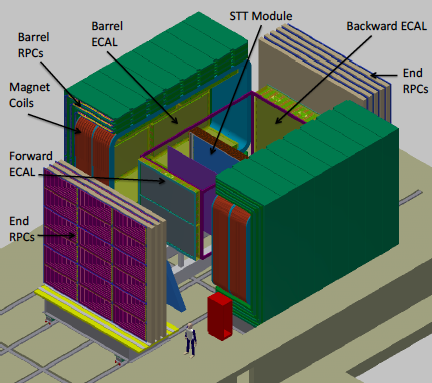
\includegraphics[width=12cm]{DUNENearDetector.png}
  \caption[Schematic of the DUNE near neutrino detector fine-grained tracker design.]{Schematic of the DUNE near neutrino detector fine-grained tracker design \cite{DUNECDR4}.}
  \label{fig:DUNENearDetector}
\end{figure}

The STT consists of over 107,000 tubes made from carbon and aluminium and with outer diameter 1~cm to provide fine-grained tracking (thickness $<0.1X_0$) with excellent angular and spatial resolution.  The tubes will be filled with either 70\% Ar, 30\% CO$_2$ or 70\% Xe, 30\% CO$_2$ depending on the positioning of the tubes in the detector and are read out at both ends.  Nuclear targets will be placed upstream with multiple materials used to make complimentary measurements.  Pressurised argon gas or calcium will allow nuclear effects of neutrino interactions on argon and modelling of signals and backgrounds in the DUNE far detector.  Carbon (graphite) may also be used to study interactions on free protons and H$_2$O and D$_2$O targets will allow analysis of interactions on quasi-free neutrinos via statistical subtractions.

The ECAL provides high segmentation in both the transverse and longitudinal directions and is composed of three separate systems; Forward ECAL, Barrel ECAL and Backward ECAL.  It is designed to reconstruct photons from $\pi^0$ decay and electrons and positrons from Bremsstrahlung radiation and consists of layers of either 1.75~mm thick (Forward ECAL) or 3.5~mm thick (Barrel and Backward ECALs) lead sheets positioned within 2.5~cm wide, 10~mm thick plastic scintillator bars.

The 0.4~T magnet has inner dimensions 4.5~m wide, 4.5~m high, 8.0~m long and assists with measurements of particle momentum and charge.  It is also instrumented with the MuIDs designed to distinguish muons from hadrons utilising the ability of muons to penetrate the iron without showering or interacting.  The MuID is comprised of 432 resistive plate chamber (RPC) modules distributed within two 10~cm thick steel plates of the magnet and will also perform basic reconstruction on the muon track segments which can be matched with tracks from the STT tracker for global object reconstruction.

%----------------------------------------------------------------------------------------------------------------------------------------------------------------------------
\subsubsection{Beamline Measurement System}\label{sec:BLM}

The beamline measurement system will operate for the life of the experiment and will monitor the beam profile on a spill-by-spill basis.  Along with constraining the neutrino flux, it will be used to monitor the pulse-to-pulse variations for beam diagnostics.  It will make measurements of the muons exiting the decay pipe originating from the meson decays which created the neutrinos in the beam.  This provides an independent measure of the muon neutrino flux and an additional handle on beam electron neutrinos resulting from muon decays.  The measurements are also useful in validating the simulation of the thick target, horn material, decay tunnel and absorber.

%----------------------------------------------------------------------------------------------------------------------------------------------------------------------------
\section{The Physics of DUNE}\label{sec:DUNEPhysics}

The staged approach to the DUNE experiment will allow early preliminary results but will require more time for facilities from later phases to be constructed and commissioned.  For this and other reasons, the accumulated data is often referred to as an `exposure', a function of detector size, beam power and time with units kt$\cdot$MW$\cdot$year.  The current assumptions on exposures for the first few years of operation are shown in Table~\ref{tab:DUNEExposure}.  This staging will be assumed in all sensitivities presented in this section.

\begin{table}
  \caption{Exposures anticipated for the DUNE experiment for the first few years of operation.  Due to the staged approach in construction, it will take some time to reach full design capabilities.  The first exposure column represents the exposure expected in that year and the next column the cumulative total.  Adapted from \cite{DUNECDR1}.}
  \label{tab:DUNEExposure}
  \centering
  \begin{tabular}{ >{\raggedright\arraybackslash}m{1.5cm} >{\raggedright\arraybackslash}m{2.5cm} >{\raggedright\arraybackslash}m{2.5cm} >{\raggedright\arraybackslash}m{7cm} }
    \toprule
    Year & Exposure (kt$\cdot$MW$\cdot$year) & Total (kt$\cdot$MW$\cdot$year) & Detector stage \\[1ex]
    \midrule
    Year 1 & 10.7 & 10.7  & 10~kt far detector, no near detector, 1.07~MW 80~GeV proton beam ($1.47\times10^{21}$ pot per year) \\[1ex]
    Year 2 & 21.4 & 32.1  & Addition of second 10~kt far detector module \\[1ex]
    Year 3 & 32.1 & 64.2  & Addition of third 10~kt far detector module and initial constraints from near detector \\[1ex]
    Year 4 & 42.8 & 107.0 & Addition of fourth 10~kt far detector module \\[1ex]
    Year 5 & 42.8 & 149.8 & Inclusion of constraints from full near detector data analysis \\[1ex]
    Year 7 & 85.6 & 278.2 & Upgrade beam power to 2.14~MW for 80~GeV proton beam \\[1ex]
    \bottomrule
  \end{tabular}
\end{table}

The appearance probability expected at the DUNE far detector is demonstrated in Figure~\ref{fig:DUNEAppearanceProbabilities} for various values of $\delta_{\textnormal{CP}}$.  It can be seen why a broadband beam with the ability to operate in neutrino and antineutrino mode mode is critical; the value of $\delta_{\textnormal{CP}}$ affects both the frequency and amplitude of the oscillations, with differing effects at the distinct oscillation nodes and between neutrinos and antineutrinos.

\begin{figure}
  \centering
  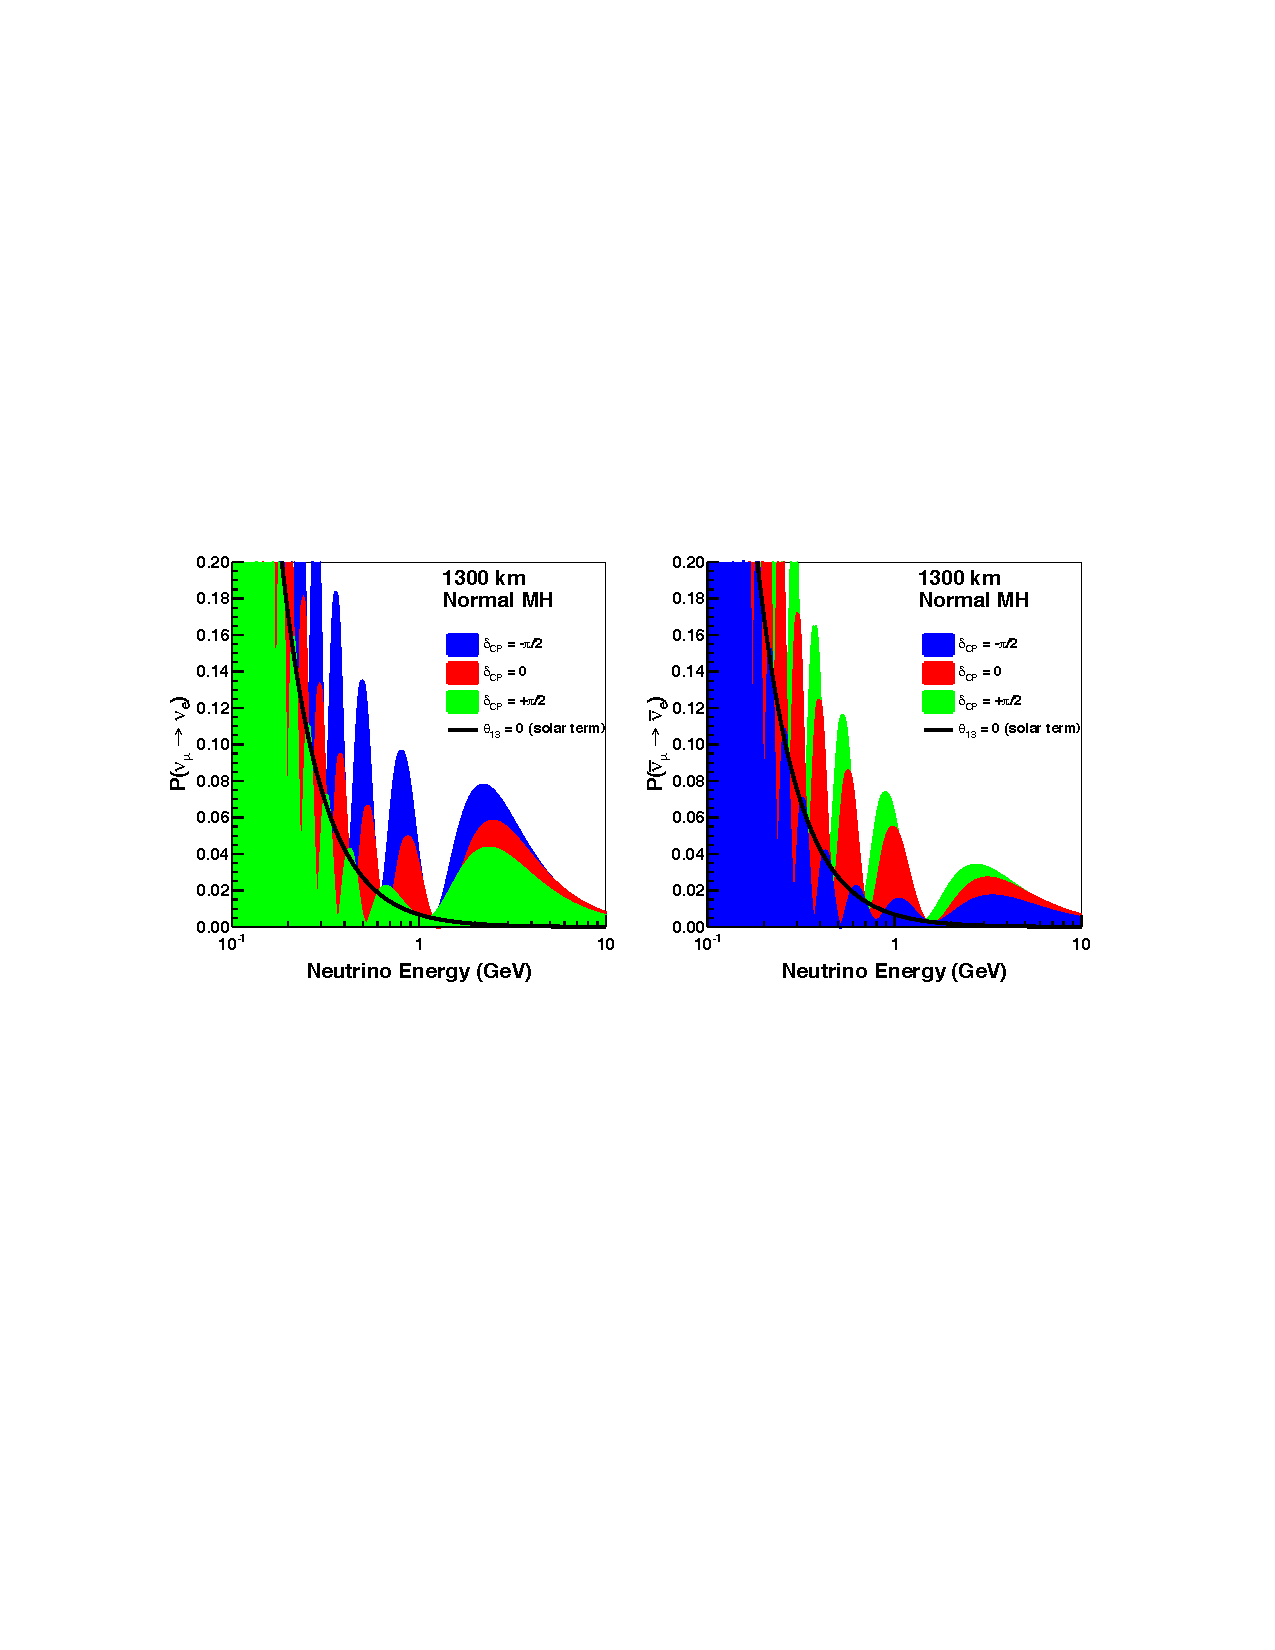
\includegraphics[width=16cm]{DUNEAppearanceProbabilities.pdf}
  \caption{The appearance probability at a baseline of 1300~km, as a function of neutrino energy, for $\delta_{CP}=-\pi/2$ (blue), 0 (red) and $\pi/2$ (green) for neutrinos (left) and antineutrinos (right), for normal hierarchy.  The black lines indicates the oscillation probability if $\theta_{13}$ were equal to zero.  Taken from \cite{DUNECDR2}.}
  \label{fig:DUNEAppearanceProbabilities}
\end{figure}

%----------------------------------------------------------------------------------------------------------------------------------------------------------------------------
\subsection{Mass Hierarchy and CP Violation}\label{sec:DUNEMassHierarchyCPViolation}

The measurements of the mass hierarchy and the degree of CP violation are determined by simultaneously fitting the $\nu_{\mu}\rightarrow\nu_{\mu}$, $\bar{\nu}_{\mu}\rightarrow\bar{\nu}_{\mu}$, $\nu_{\mu}\rightarrow\nu_e$ and $\bar{\nu}_{\mu}\rightarrow\bar{\nu}_e$ oscillated spectra, assuming 50\% neutrino, 50\% antineutrino exposure.

The sensitivity of DUNE to the neutrino mass hierarchy is shown in Figure~\ref{fig:DUNEMassHierarchy}.  It is evident DUNE will discover the ordering of the mass states at $5\sigma$ significance within the first few years of running, regardless of the value of $\delta_{\textnormal{CP}}$.  This is achievable because of the large matter effects present with a 1300~km baseline; the asymmetry between neutrinos and antineutrinos due to this is approximately $\pm40$\% in the region of peak flux.

\begin{figure}
  \centering
  \begin{subfigure}[t]{\linewidth}
    \centering
    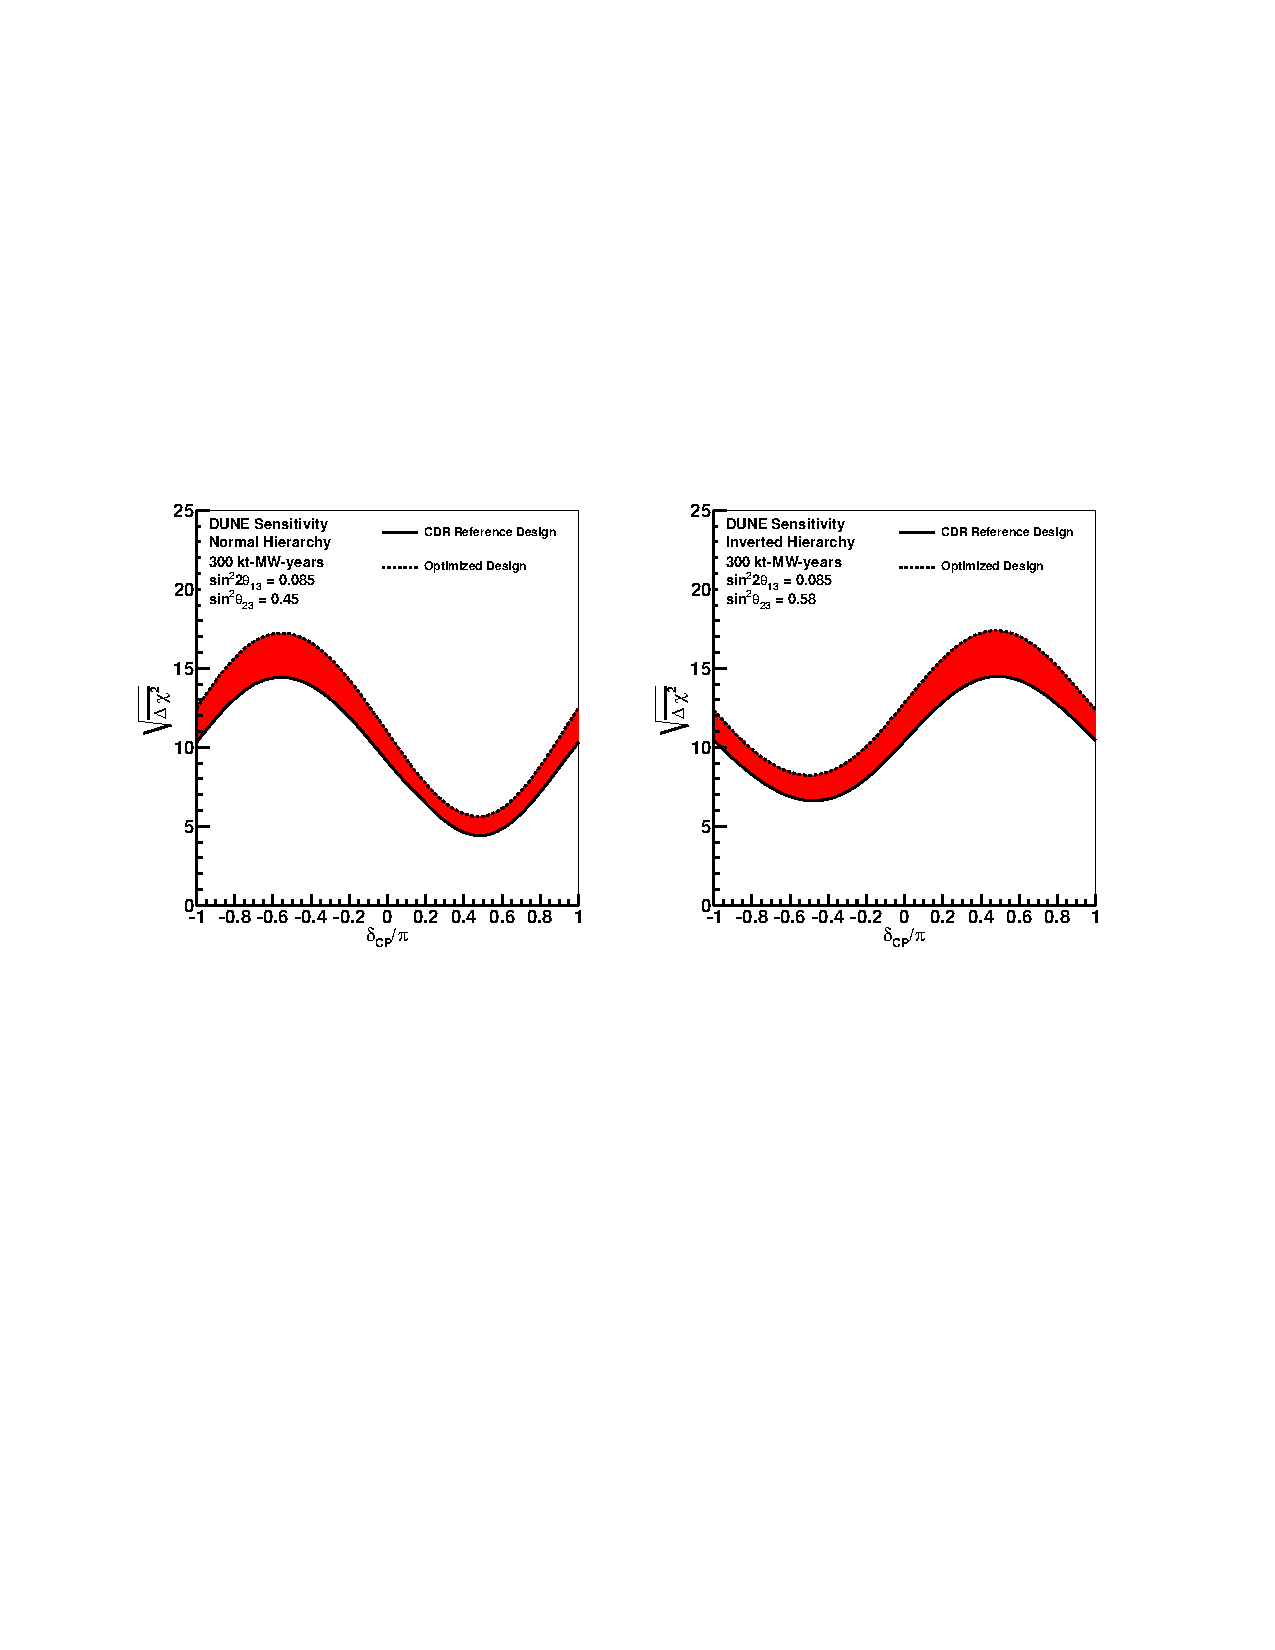
\includegraphics[width=16cm]{DUNEMassHierarchyDeltaCP.pdf}
    \caption{The significance with which the mass hierarchy can be determined as a function of the value of $\delta_{CP}$ for an exposure of 300~kt$\cdot$MW$\cdot$year assuming normal hierarchy (left) and inverted hierarchy (right).  Taken from \cite{DUNECDR2}.}
    \label{fig:DUNEMassHierarchyDeltaCP}
  \end{subfigure}
  \hfill
  \vfill
  \begin{subfigure}[t]{\linewidth}
    \centering
    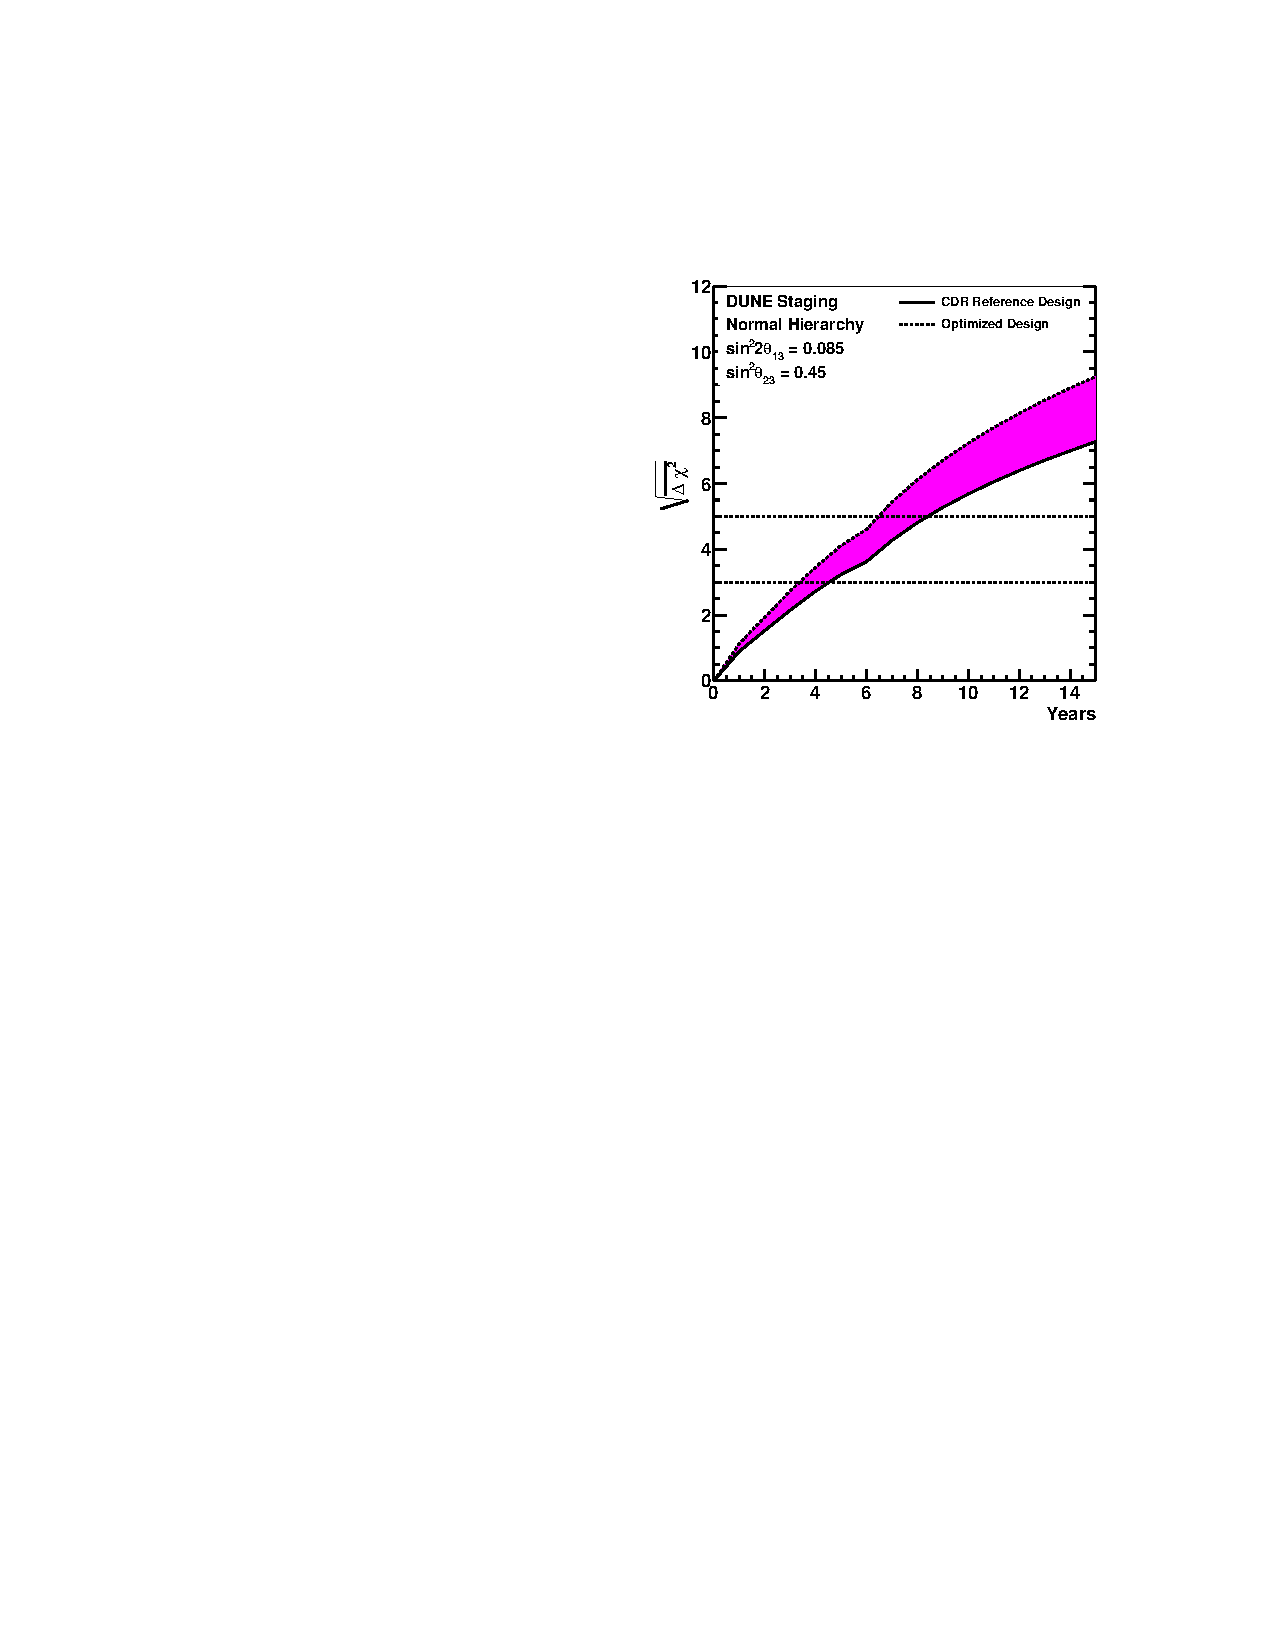
\includegraphics[width=8cm]{DUNEMassHierarchyTime.pdf}
    \caption{Assuming normal hierarchy, the minimum significance (the lowest point on the curve in Figure~\ref{fig:DUNEMassHierarchyDeltaCP}) with which the mass hierarchy can be determined for all values of $\delta_{CP}$ as a function of years of running under the assumptions in Table~\ref{tab:DUNEExposure}.  Taken from \cite{DUNECDR1}.}
    \label{fig:DUNEMassHierarchyTime}
  \end{subfigure}
  \caption[Sensitivity of the DUNE experiment to the neutrino mass hierarchy.]{Sensitivity of the DUNE experiment to the neutrino mass hierarchy.}
  \label{fig:DUNEMassHierarchy}
\end{figure}

The equivalent sensitivities for CP violation is displayed in Figure~\ref{fig:DUNECPViolation}.  It is impossible to cover 100\% of $\delta_{\textnormal{CP}}$ values because, in the case of CP conservation, the violation effects (i.e. disparities between neutrino and antineutrino oscillations) disappear.  DUNE will be able to measure 75\% of possible $\delta_{\textnormal{CP}}$ values with 3$\sigma$ significance after 1320~kt$\cdot$MW$\cdot$year and, in the case of near-maximal CP violation currently hinted at by T2K \cite{T2K2017}, 50\% of these large CP-violating $\delta_{\textnormal{CP}}$ values will be measured at 5$\sigma$ confidence with an exposure of 810~kt$\cdot$MW$\cdot$year, around 14 years of running following the staging described in Table~\ref{tab:DUNEExposure}.  A full scope experiment operating with multi-megawatt beam power will eventually achieve around a 5\% precision of the CP-violating phase, comparable to the equivalent precision in the quark sector described in the CKM matrix.

\begin{figure}
  \centering
  \begin{subfigure}[t]{\linewidth}
    \centering
    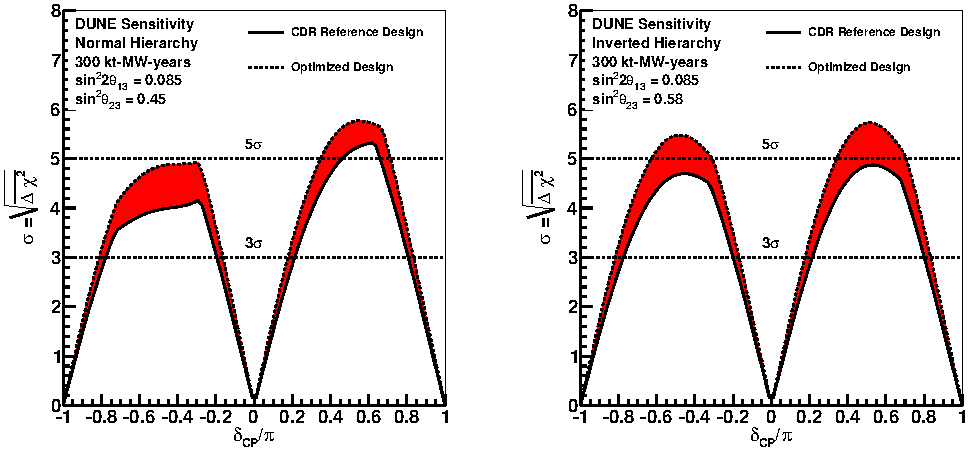
\includegraphics[width=16cm]{DUNECPViolationDeltaCP.pdf}
    \caption{The significance with which CP violation can be determined as a function of the value of $\delta_{CP}$ for an exposure of 300~kt$\cdot$MW$\cdot$year assuming normal hierarchy (left) and inverted hierarchy (right).  Taken from \cite{DUNECDR2}.}
    \label{fig:DUNECPViolationDeltaCP}
  \end{subfigure}
  \hfill
  \vfill
  \begin{subfigure}[t]{\linewidth}
    \centering
    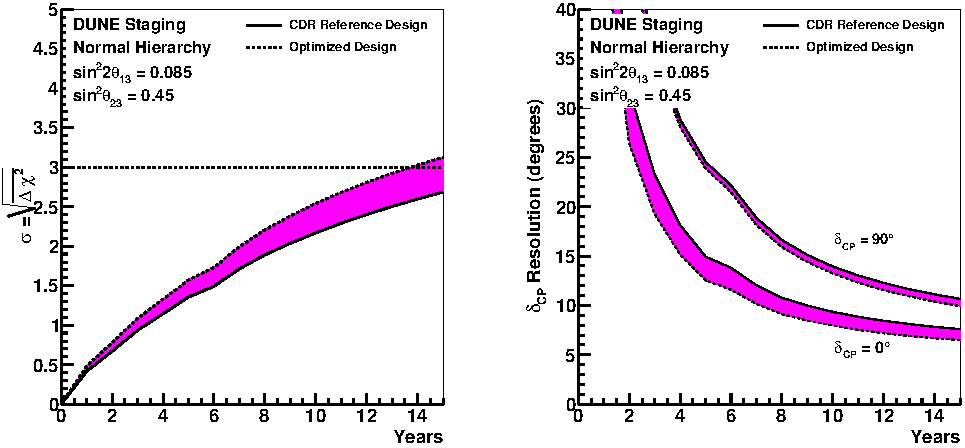
\includegraphics[width=16cm]{DUNECPViolationTime.pdf}
    \caption{Assuming normal hierarchy, the significance with which CP violation can be determined for 75\% of $\delta_{\textnormal{CP}}$ values (left) and the expected 1$\sigma$ resolution (right) as a function of years of running under the assumptions in Table~\ref{tab:DUNEExposure}.  Taken from \cite{DUNECDR1}.}
    \label{fig:DUNECPViolationTime}
  \end{subfigure}
  \caption[Sensitivity of the DUNE experiment to leptonic CP violation.]{Sensitivity of the DUNE experiment to leptonic CP violation.}
  \label{fig:DUNECPViolation}
\end{figure}

%----------------------------------------------------------------------------------------------------------------------------------------------------------------------------
\subsection{Oscillation Parameters}\label{sec:DUNEOscillationParameters}

DUNE will make precision measurements of all parameters describing neutrino oscillations and improve our understanding of oscillation phenomenology.  The least known mixing angle, $\theta_{23}$, will be measured with a precision of at least 1$^{\circ}$, even near 45$^{\circ}$.  This is possible by performing a combined analysis of the $\nu_{\mu}\rightarrow\nu_{\mu}$ and $\nu_{\mu}\rightarrow\nu_e$ channels, proportional to $\sin^2{2\theta_{23}}$ and $\sin^2{\theta_{23}}$ respectively (from Equations~\ref{eq:MuonNeutrinoDisappearance} and~\ref{eq:ElectronNeutrinoAppearance}).  The sensitivity of DUNE to the octant of $\theta_{23}$, and the resolution of the value itself, is presented in Figure~\ref{fig:DUNETheta23}.  The current world-leading measurements of $\theta_{13}$ from reactor experiments will also be achieved after sufficient exposure in the DUNE experiment, using analyses of $\nu_e$ and $\bar{\nu}_e$ appearance.  The resolution of this, along with the anticipated resolution of the associated mass splitting, $\Delta m_{31}^2$, are shown in Figure~\ref{fig:DUNETheta13}.

\begin{figure}
  \centering
  \begin{subfigure}[t]{0.48\linewidth}
    \centering
    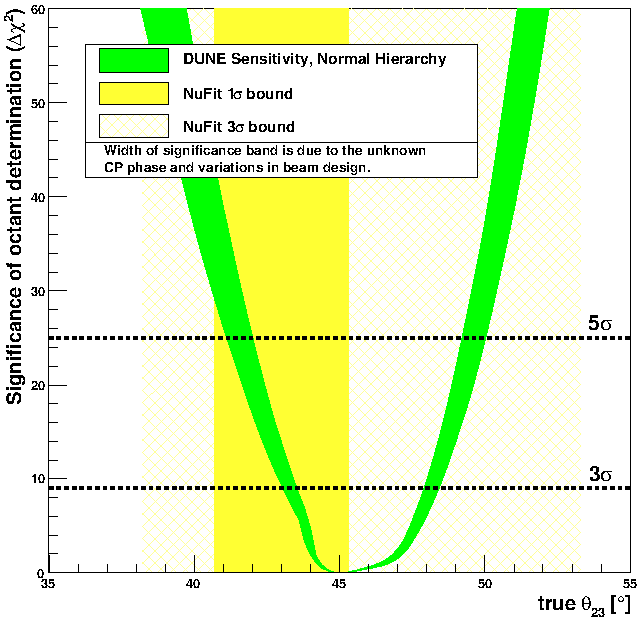
\includegraphics[width=0.98\textwidth]{DUNEOctantSensitivity.pdf}
    \caption{DUNE octant sensitivity.}
    \label{fig:DUNEOctantSensitivity}
  \end{subfigure}
  \hfill
  \begin{subfigure}[t]{0.48\linewidth}
    \centering
    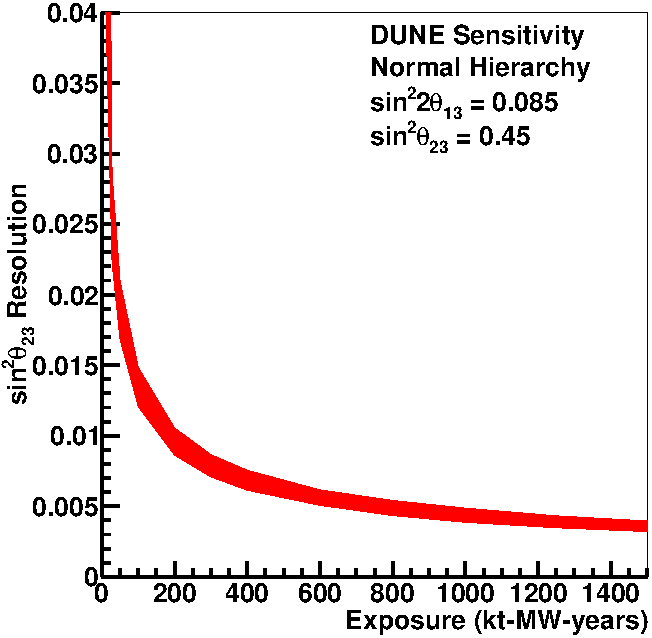
\includegraphics[width=0.98\textwidth]{DUNETheta23Resolution.pdf}
    \caption{DUNE $\sin^2{\theta_{23}}$ resolution.}
    \label{fig:DUNETheta23Resolution}
  \end{subfigure}
  \caption[The sensitivity of DUNE to the octant and value of $\theta_{23}$.]{The sensitivity of DUNE to the octant and value of $\theta_{23}$.  Figure~\ref{fig:DUNEOctantSensitivity} shows the significance with which DUNE can resolve the $\theta_{23}$ octant as a function of the true value of $\theta_{23}$.  The green shaded band around the curve represents the range in sensitivity due to potential variations in the beam design and in the true value of $\delta_{\textnormal{CP}}$.  The yellow shaded regions indicate the current 1$\sigma$ and 3$\sigma$ bounds on the value of $\theta_{23}$ from a global fit.  An exposure of 1320~kt$\cdot$MW$\cdot$year, which will provide a 3$\sigma$ measurement of CP violation for 75\% of the values of $\delta_{\textnormal{CP}}$ is assumed.  Figure~\ref{fig:DUNETheta23Resolution} shows the resolution of a measurement of $\sin^2{\theta_{23}}$ as a function of exposure assuming normal mass hierarchy and $\sin^2{\theta_{23}}=0.45$ from the current global fit.  The shaded region represents the range in sensitivity due to potential variations in the beam design.  Taken from \cite{DUNECDR2}.}
  \label{fig:DUNETheta23}
\end{figure}

\begin{figure}
  \centering
  \begin{subfigure}[t]{0.48\linewidth}
    \centering
    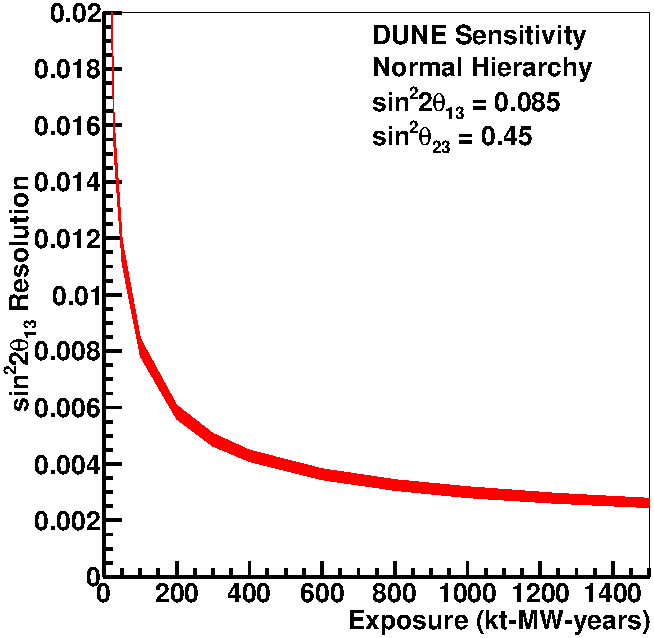
\includegraphics[width=0.98\textwidth]{DUNETheta13Resolution.pdf}
    \caption{DUNE $\sin^2{2\theta_{13}}$ resolution.}
    \label{fig:DUNETheta13Resolution}
  \end{subfigure}
  \hfill
  \begin{subfigure}[t]{0.48\linewidth}
    \centering
    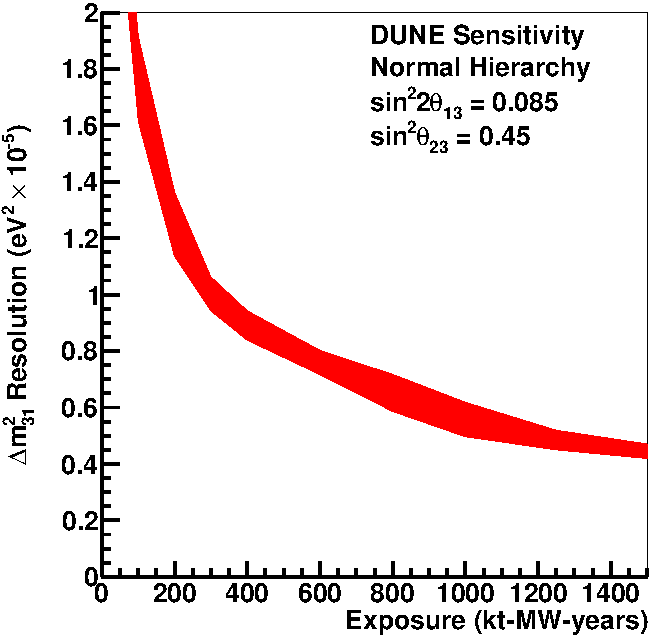
\includegraphics[width=0.98\textwidth]{DUNEDeltaM31Resolution.pdf}
    \caption{DUNE $\Delta m_{31}^2$ resolution.}
    \label{fig:DUNEDeltaM31Resolution}
  \end{subfigure}
  \caption[The sensitivity of DUNE to the oscillation parameters describing $\nu_e$ and $\bar{\nu}_e$ appearance.]{The sensitivity of DUNE to the oscillation parameters describing $\nu_e$ and $\bar{\nu}_e$ appearance as a function of exposure assuming normal hierarchy.  Figure~\ref{fig:DUNETheta13Resolution} shows the resolution of a measurement of $\sin^2{2\theta_{13}}$ and Figure~\ref{fig:DUNEDeltaM31Resolution} shows the resolution of $\Delta m_{31}^2$ assuming, from current global fits, $\sin^2{2\theta_{13}}=0.085$ and $\Delta m_{31}^2=2.457\times10^{-3}$~eV$^2$.  The shaded regions represent the range in sensitivity due to potential variations in the beam design.  Taken from \cite{DUNECDR2}.}
  \label{fig:DUNETheta13}
\end{figure}

%----------------------------------------------------------------------------------------------------------------------------------------------------------------------------
\subsection{Other Physics}\label{sec:DUNEOtherPhysics}

The LBNF/DUNE physics program is diverse and contains priorities unrelated to beam neutrino physics.  These are not wholly relevant to this thesis and shall not be discussed in detail but it would be inappropriate to ignore the additional physics potential of the experiment.

The capabilities to search for nucleon decay, mainly via the $p\rightarrow K^+\bar{\nu}$ channel, will improve lifetime limits by an order of magnitude after 20 years' running.  It will significantly extend sensitivities compared to water Cherenkov detectors as a consequence of a higher detection efficiency and low background rates.  Many models in which this mode is dominant (e.g. supersymmetric GUT models) also favour other models with final-state kaons, enabling a wide range of nucleon decay physics to be studied at the DUNE far detector.

The unique sensitivity to supernova $\nu_e$ neutrinos, via the interaction
\begin{equation}
  \nu_e + ^{40}\textnormal{Ar} \rightarrow e^- + ^{40}\textnormal{K}^*, \\
\end{equation}
inaccessible to water or liquid scintillator detectors which detect the $\bar{\nu}_e$ component via inverse beta decay on free protons, will, along with $\bar{\nu}_e$ interactions, allow precision measurements of the composition of supernovae should one occur during the run of the experiment.  The neutrinos from a core-collapse are emitted supernova in a burst of a few tens of seconds, with around half the luminosity in the first second.  They are roughly divided equally between the three known neutrino flavours and have energies between 5-50~MeV.  A large neutrino signal from a supernova will allow unique studies of astrophysical phenomena related to the end of the lifetime of a star.

%----------------------------------------------------------------------------------------------------------------------------------------------------------------------------
\section{The Road to DUNE}\label{sec:RoadToDUNE}

The staging presented in Table~\ref{tab:DUNEExposure} is hugely ambitious and requires a great deal of preparation to ensure the project is a success.  The preparations have commenced with a program of prototyping and construction to ensure assembly of the first 10~kt module can begin as scheduled in 2021.  Work at the far detector site is underway and construction at the near detector will start next year to ensure the beam and near detector facilities are ready for 2026.

Each 10~kt module is larger than any LArTPC ever operated by well over an order of magnitude and it is crucial the detector technology is understood and the experiment operates as expected.  To ensure this is the case, a comprehensive prototyping strategy is planned.  This will be briefly overviewed in this section.

%----------------------------------------------------------------------------------------------------------------------------------------------------------------------------
\subsection{The 35~ton Prototype}\label{sec:35ton}

The first prototype to test many of the design features of the DUNE far detector was the 35~ton, shown in Figure~\ref{fig:DUNE35ton}.  This is the subject of the majority of this thesis and will be properly discussed in Chapter~\ref{chap:35ton}.  Lessons learned from the 35~ton experience are already influencing the design choices and operating schedules of the next prototypes and the far detector, highlighting the benefits of a thorough research and development program.

\begin{figure}
  \centering
  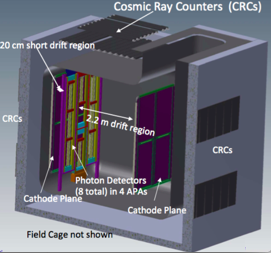
\includegraphics[width=8cm]{35ton.png}
  \caption[The 35~ton cryostat and detector designed to prototype the DUNE far detector design.]{{\color{red}Will replace this will a better image when I write the 35ton chapter.} The 35~ton cryostat and detector designed to prototype the DUNE far detector design.}
  \label{fig:DUNE35ton}
\end{figure}

The 35~ton experiment demonstrated the cryostat and detector technologies over the course of two runs, in early 2014 and early 2016 respectively, by collecting and analysing data from cosmic-induced tracks and showers.  Analysis of data from the second run is the subject of Chapter~\ref{chap:35tonAnalysis}.

%----------------------------------------------------------------------------------------------------------------------------------------------------------------------------
\subsection{ProtoDUNE}\label{sec:ProtoDUNE}

The next prototypes, ProtoDUNE, will take data during the second half of 2018 and will be a full scale engineering prototype of the DUNE far detector.  ProtoDUNE is hosted at the Neutrino Platform at CERN and consists of two demonstrators utilising single-phase (ProtoDUNE-SP) \cite{ProtoDUNE-SP} and dual-phase (ProtoDUNE-DP) \cite{WA105} designs.  The layout is shown in Figure~\ref{fig:NeutrinoPlatform}.  The cryostats contain more than 700~t LAr and represent an intermediary stage between the 35~ton and the DUNE far detector modules.

\begin{figure}
  \centering
  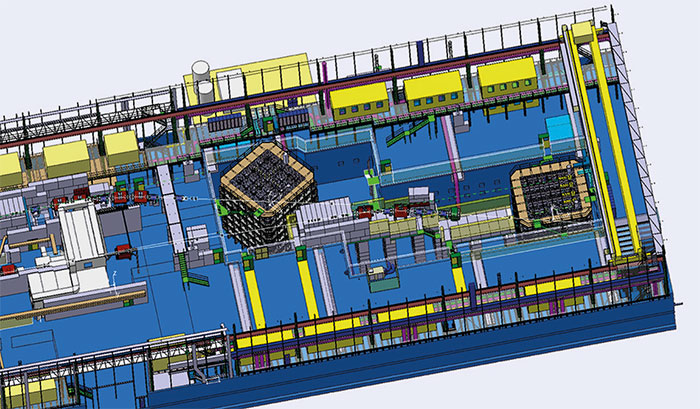
\includegraphics[width=14cm]{NeutrinoPlatform.jpg}
  \caption[Schematic showing the layout of the ProtoDUNEs at the CERN neutrino platform.]{Schematic showing the layout of the ProtoDUNEs at the CERN neutrino platform \cite{NeutrinoPlatform}.  The cryostat at the left, on a slight angle, is the dual-phase LArTPC and the single-phase detector is at the right hand side.  The beamline, running from left to right through both detectors, is evident.}
  \label{fig:NeutrinoPlatform}
\end{figure}

The detectors are being constructed in a CERN test beam and will be subjected to various particles, including $e^{\pm}, \mu^{\pm}, K^{\pm}, p, \bar{p}$.  Along with characterising the detector performance and identifying potential improvements, ProtoDUNE will provide calibrations, such as electromagnetic shower energy resolution, electron/photon separation and particle identification, for the far detector and facilitate an assessment of the detector systematics.  It will also provide opportunity, in a detector functionally identical to the far detector modules, to validate the simulation and reconstruction techniques developed in Monte Carlo.  Upon completion of the ProtoDUNE program, DUNE will be prepared to begin final preparations and construction of the first, single-phase, far detector module.

%----------------------------------------------------------------------------------------------------------------------------------------------------------------------------
%% \subsection{Towards DUNE}\label{sec:TowardsDUNE}
